\documentclass[12pt]{article}
\usepackage{amsmath, amsthm, amssymb, graphicx, verbatim}

\setlength\topmargin{0in}
\setlength\headheight{-.5in}
\setlength\headsep{0in}
\setlength\textheight{9.75in}
\setlength\textwidth{7.3in}
\setlength\oddsidemargin{-.5in}
\setlength\evensidemargin{-.5in}
\setlength\footskip{1in}

\newtheorem{theorem}{Theorem}
\newtheorem{lemma}[theorem]{Lemma}
\newtheorem{proposition}[theorem]{Proposition}
\newtheorem{corollary}[theorem]{Corollary}
\newtheorem{definition}[theorem]{Definition}

\def \sp{\spadesuit}
\def \cl{\clubsuit}
\def \he{\heartsuit}
\def \di{\diamondsuit}


\title{Notes - Math 135b}

\begin{document}
\maketitle
\section*{3/30}
  \subsection*{Limit Theorems}
    Given a sequence of random variables, $Y_1, Y_2, \ldots$,
    we want to show that "when $n$ is large", $Y_n$ is approximately $f(n)$ for 
    some simple (deterministic) function, $f(n)$.
    \begin{definition}
      A sequence, $Y_1, Y_2, \ldots$, of random variables converges to a number,
      $a$, \underline{in probability} if $P(|Y_n - a| \le \epsilon)$ converges
      to 1 for any fixed $\epsilon$. This is equivalent to $P(|Y_n - a| > 
      \epsilon)$ converges to 0.
    \end{definition}
    \underline{Example}:\\
      \begin{enumerate}
        \item Let $X_1, X_2, \ldots$ be a sequence of independent and identically
          distributed (iid) numbers.\\
          $EX_i = \mu$ and $Var(X_i) = \sigma^2$.\\
          $S_n = X_1 + \ldots + X_n$.\\
          When $n$ is large, $\frac{S_n}{n\mu}$ converges to 1 in probability.
        \item Toss a fair coin $n$ times (independently).\\
          Let $R_n$ be the "longest runs of heads" or longest substring of 
          consecutive results of heads. (Results look like HHTTHHHTHTHTHH. 
          $R_n = 3$ in this case.)\\
          \begin{eqnarray*}
            P(R_n \ge 1) & = & P(\text{at least $k$ consecutive result of heads
              somewhere in the result string})\\
            & = & P(\bigcup_{i = 1}^{n - k + 1}) \text{ \{$i$ is the first head in an
              interval of at least $k$ heads\}}\\
            & \le & n \frac{1}{2^k} 
          \end{eqnarray*}
          We discovered the upper bound. Now, for the lower bound.\\
          Divide the string of size $n$ instead disjoint strings of size $k$i.
          \begin{eqnarray*}
            P(R_n \ge k) & \le & P(\text{at least one of the blocks consists of
              all heads})\\
              & = & 1 - (1 - \frac{1}{2^k})^{\lfloor\frac{n}{k}\rfloor}
          \end{eqnarray*}
      \end{enumerate}
      \begin{theorem}
        $\frac{R_n}{\log_2n}$ converges to 1 in probability
      \end{theorem}

\section*{4/1}
  From last time,
  Let there be $n$ tosses of a fair coin and $R_n$ be the longest interval of 
  heads.\\
  $$
    P(R_n \ge k) \le n \frac{1}{2^k}
  $$
  $$
    P(R_n \ge k) \ge 1 - \left(1 - \frac{1}{2^k}\right)^{\lfloor \frac{n}{k}\rfloor}
  $$
  \begin{theorem}
    $$
      \frac{R_n}{\log_2n} \to 1
    $$
    in probability
  \end{theorem}
  \begin{proof}
    Need to show that for any $\epsilon > 0$
    \begin{eqnarray}
      P(R_n \ge (1 + \epsilon) \log_2n) & \to & 0\\
      P(R_n \ge (1 - \epsilon) \log_2n) & \to & 1 
    \end{eqnarray}
    \begin{eqnarray*}
      P\left(\left|\frac{R_n}{\log_2n} - 1\right| \ge \epsilon\right)
      & = & P\left(\frac{R_n}{\log_2n} \ge 1 + \epsilon \text { or } 
      \frac{R_n}{\log_2n} \le 1 - \epsilon\right)\\
      & = & P\left(\frac{R_n}{\log_2n} \ge 1 + \epsilon\right) + P\left(\frac{R_n}{
      \log_2n} \le 1 - \epsilon\right)\\
    \end{eqnarray*}
    Plug in $k = (1 + \epsilon)\log_2n$ to equation (1), you get
    \begin{eqnarray*}
      \ldots & \le & n \frac{1}{2^{(1 + \epsilon)\log_2n}}\\
      & = & n \frac{1}{n^{1 + \epsilon}}\\
      & = & \frac{1}{n^{\epsilon}}
    \end{eqnarray*}
    Plug in $k = (1 - \epsilon)\log_2n$ to equation (2), you get
    \begin{eqnarray*}
      \ldots & \ge & 1 - e^{-\frac{1}{2^k} \lfloor\frac{n}{k}\rfloor}\\
      & \ge & 1 - e^{\frac{-1}{2^k}(\frac{n}{k} - 1)}\\
      & \ge & 1 - exp(-n^{-(1 - \epsilon)}(\frac{n}{(1 - \epsilon)\log_2n) - 1}\\
      & = & 1 - exp\left(- n^{\epsilon}\frac{1}{(1 - \epsilon)\log_2n} + \frac{1}{n^{1 - \epsilon}}\right)\\
      & \to & 1
    \end{eqnarray*}
  \end{proof}
  \begin{theorem}[Markov's inequality]
    If $X \ge 0$ is any random variables, $P(X > a) \le \frac{1}{a}EX$
  \end{theorem}
  \begin{proof}
    $I\{X \ge a\}$ where this is 1 when the event happens and 0 otherwise.
    $I\{X \ge a\} \le \frac{1}{a}X$ by Bernoulli
  \end{proof}
  \begin{theorem}[Chebyshev's inequality]
    $EX = \mu$ and $Var(X) = \mu^2$. Otherwise, $X$ is aribitrary.\\
    Then, 
    \begin{eqnarray*}
      P(|X - \mu| \ge k) & \le & \frac{\sigma^2}{k^2}\\
      P((X - \mu)^2 \ge k^2)& \le & \frac{\sigma^2}{k^2}
    \end{eqnarray*}
  \end{theorem}
  \begin{proof}
    We need to prove
    \begin{eqnarray*}
      P\left(\left|\frac{S_n}{n} - \mu\right|\ge \epsilon\right) & \to & 0\\
      E\left(\frac{S_n}{n}\right) & = & \frac{1}{n} n\mu = \mu\\
      Var\left(\frac{S_n}{n}\right)
    \end{eqnarray*}
    $$
      S_n = X_1 + \ldots + X_n \text{ where $X_i$ is aribtrary}
    $$ 
    $$
      ES_n = EX_1 + \ldots + EX_n
    $$
    \begin{eqnarray*}
      Var(S_n) & = & Var(X_1) + \ldots + Var(X_n) + \sum_{i \not= j}Cov(X_i, X_j)\\
      Cov(X_1, X_j) & = & E(X_iX_j) - EX_i EX_j\\
      Var(aX) = a^2(n
    \end{eqnarray*}
  \end{proof}
  \begin{theorem}[Weak law of large numbers]
    Let $X_1, X_2, \ldots$ be a sequence that is iid with $EX_1 = \mu$ and
    $Var(X_1) = \sigma^2 < \infty$.\\
    $S_n = X_1 + \ldots + X_n$\\
    Then, $\frac{S_n}{n} \to \mu$ in probability.
  \end{theorem}
  \begin{proof}
    Rest on the two inequalities:
    \begin{eqnarray*}
      P\left(\left|\frac{S_n}{n} - \mu\right| \ge \epsilon\right) 
      & \le & \frac{1}{\epsilon^2}\cdot \frac{\sigma^2}{n}\\
      & \to & 0
    \end{eqnarray*}
  \end{proof}
  \underline{example}: Two investment choices at the beginning of each year:
    \begin{itemize}
      \item a risk-free "bond" which returns 6\% per year
      \item a risky "stock" which increases your investment by 50\% with
        probability .8 and wipes away your money with probability .2
    \end{itemize}
    If your money is $s$, then after a year, bond will give you $1.06s$
    and stock $\begin{cases} 1.5s & \text{ with probability .8}\\
    0 & \text{ with probabiliy .2}\end{cases}$

\section*{4/3}
  "hedging" - invest a fixed proportion $x$ into the stock and
  $1 - x$ into the bond. (We know that when $x = 1$, you will 
  eventually lose everything.)\\
  Average growth is
  $$
    \lambda = \lim_{n \to \infty} \frac{1}{n} \log\frac{x_n}{x_0}
  $$
  where $x_n \approx x_0 e^{\lambda n}$.\\
  $x_n$ is your capital at the end of year $n$.\\
  $I_i = I\{$ stocks goes up in year $i \}$.\\
  They are independent indicators with $EI_i = .8$.\\
  \begin{eqnarray*}
    x_n & = & x_{n-1}(1-x)\cdot 1.06 + x_{n-1} \cdot x \cdot 1.5 \cdot I_n\\
      & = & x_{n-1}(1.06(1 - x) + 1.5x \cdot I_n)\\
      & = & x_0(1.06(1-x) + 1.5x)^{s_n}((1 - x)1.06)^{n - s_n} 
        \text{ where } s_n = I_1 + \ldots I_n\\
  \end{eqnarray*}
  The last step unrolled the recurrence.\\
  \begin{eqnarray*}
    \frac{1}{n}\log\frac{x_n}{x_0} & = & \frac{s_n}{n} \log(1.06 + .44x)
      + (1 - \frac{S_n}{n})\log(1.06(1-x))\\
      & \to_{n \to \infty} & .8 \log(1.06 + .44x) + .2 \log(1.06(1 - x))\\
  \end{eqnarray*}
  To maximize this,
  $$
    \frac{.8 \cdot .44}{1.06 + .44x} = \frac{.2}{1-x}
  $$
  where $x \in (0,1)$
  Therefore,
  $\lambda = \lim_{n \to \infty} \frac{1}{n}\log\frac{x_n}{x_0}$ where
  $x_n \approx x_0 e^{n\lambda}$.\\\\
  $e^{\lambda} = 1 + u$\\
  Solve $x = \frac{7}{22}$ and $\lambda \approx 8.1\%$ and $u = 8.4\%$\\\\
\underline{Example}:  Distribute $n$ balls independently at random into
  $n$ boxes. $N_n$ is the number of empty boxes.\\
  $N_n = I_1 + \ldots + I_n$ where $I_i = I\{ i$th box is empty$\}$\\
  You would use weak law of large number, but they're not independent.\\
  $$
    EI_i = \left(\frac{n-1}{n}\right)^n = \left(1 - \frac{1}{n}\right)^n \to e^{-1}
  $$
  $$
    E(N_n^2) = EN_n + \sum_{i \not= j} E(I_iI_j)
  $$
  $$
    E(I_iI_j) = P(\text{both box $i$ and $j$ are empty}) = \left(\frac{n - 2}{n}\right)^n
  $$
  $$
    Var(N_n) = E(N_n^2) - (EN_n)^2 = n\left(1 - \frac{1}{n}\right)^n + 
    n(n-1)\left(1 - \frac{2}{n}\right)^n - n^2 \left(1 - 
    \frac{1}{n}\right)^{2n}
  $$
  By chebyshev's inequality,
  \begin{eqnarray*}
    P\left(\left|\frac{1}{n}N_n - \frac{1}{n}EN_n\right| \ge \epsilon\right)
      & \le & \frac{1}{\epsilon^2} \frac{1}{n^2} VarN_n\\
      & = & \frac{1}{\epsilon^2}\left(\frac{1}{n}\left(1 - \frac{1}{n}\right)^n 
        + \frac{n-1}{n}\left(1 - \frac{2}{n}\right)^n - \left(1 - 
        \frac{1}{n}\right)^{2n}\right)\\
      & \to_{n \to \infty} & \frac{1}{\epsilon^2}(0 + e^{-2} - e^{-2})\\
      & = & 0
  \end{eqnarray*}
  This implies that $P\left(\left|\frac{1}{n}N_n - e^{-1}\right| > 
  \epsilon \right) \to 0$

\subsection*{Moment Generating functions and Central Limit Theorems}
  If $X$ is a random variable, then its \underline{moment generating 
  function} is 
  $$
    \phi(t) = \phi_X(t) = E(e^{tX}) = 
    \begin{cases} 
      \sum_x e^{tx} P(X=x) & \text{ discrete}\\
      \int_{-\infty}^{\infty} e^{tx} f_X(x) \,dx & \text{ continuous}\\
    \end{cases}
  $$

\section*{4/6}
  \subsection*{Moment generating function}
    $$
      \phi(t) = E[e^{tX}] = 
        \begin{cases}
          \sum_{x}e^{tX}P(X=x) & \text{discrete}\\
          \int_{-\infty}^{\infty}e^{tX}f(x)\,dx & \text{continuous}\\
        \end{cases}
    $$
    \underline{Notes}: 
    \begin{enumerate}
      \item It doesn't always exists, i.e.
      $$
        f_X(x) = 
        \begin{cases}
          e^{-x} & x > 0\\
          0 & x \le 0
        \end{cases}
      $$
      Therefore,
      $$
        \phi(t) = \int_0^{\infty}e^{tx}e^{-x}\,dx = \frac{1}{1-t}
      $$
      only when $t < 1$.
      \item 
      \begin{eqnarray*}
        E(e^{tX}) 
        & = & E[1 + tX + \frac{1}{2}t^2x^2 + \frac{1}{6} t^3x^3 + \ldots]\\
        & = & 1 + tE(X) + \frac{1}{2}t^2E(X^2) + \ldots
      \end{eqnarray*}
      Each of the $E(X^i)$ are called \textit{moments}.
    \end{enumerate}
    \underline{Example}: Poisson($\lambda$)\\
      \begin{eqnarray*}
        \phi(t) 
        & = & \sum_{n = 0}^{\infty}e^{tn} \cdot \frac{\lambda^n}{n!}e^{-\lambda}\\
        & = & e^{-\lambda}\sum_{n = 0}^{\infty} \frac{(e^t\lambda)^n}{n!}\\
        & = & e^{-\lambda + \lambda e^t}\\
        & = & e^{\lambda(e^t - 1)}
      \end{eqnarray*}
    \underline{Example}: Normal
      \begin{eqnarray*}
        \phi_X(t) 
        & = & \frac{1}{\sqrt{2\pi}} \int_{-\infty}^{\infty}e^{tx}e^{-x^2/2}\,dx\\
        & = & \frac{1}{\sqrt{2\pi}}e^{\frac{1}{2}t^2}\int_{-\infty}^{\infty} e^{-\frac{1}{2}(x - t)^2}\,dx\\
        & = & e^{\frac{1}{2}t^2}\\
      \end{eqnarray*}
      $$
        -\frac{1}{2}(2tx + x^2) = \frac{1}{2}((x-t)^2 - t^2)
      $$
      \begin{lemma}
        If $X_1, X_2, \ldots, X_n$ are independent and $S_n = X_1 + \ldots + 
        X_n$, then 
        $$
          \phi_{S_n}(t) = E[e^{tS_n}] = E[e^{tX_1} \cdot e^{tX_2} \ldots 
          e^{tX_n}] = \phi_{X_1}(t) \ldots \phi{X_n}(t)
        $$
        If $X_i$ is identically distributed as $X$, then
        $$
          \phi_{S_n}(t) = [\phi_X(t)]^n
        $$
      \end{lemma}
      \begin{theorem}
        \begin{enumerate}
          \item If $\phi_X(t) = \phi_Y(t)$ for all $t$, then
            $P(X \le x) = P(Y \le x)$ for all $x$
          \item If $\phi_{X_n}(t) \to \phi_X(t)$ for all $t$,
            then $P(X_n \le x) \to P(X \le x)$ for all $x$.
        \end{enumerate}
      \end{theorem}
      
      \underline{Example}:
        Show that the sum of independent Poisson random variables
        is Poisson.\\
        \begin{tabular}{c c c}
        $X_1$ & $Poisson(\lambda_1)$ & $e^{\lambda_1}(e^t - 1)$\\
        $X_2$ & $Poisson(\lambda_2)$ & $e^{\lambda_2}(e^t - 1)$\\
        & $\vdots$ &\\
        $X_n$ & $Poisson(\lambda_n)$ & $e^{\lambda_n}(e^t - 1)$\\
        \end{tabular}

      $$
        \phi_{X_1 + \ldots + X_n}(t) = e^{(\lambda_1 + \ldots + \lambda_n)(e^t - 1)}
      $$
      where $X_1 + \ldots X_n$ is $Poisson(\lambda_1 + \ldots + \lambda_n)$\\\\
      \underline{Example}: Moment generating functions of $Binomial(n,p)$\\
        $S_n = \sum_{k = 1}^n I_k$ where $I_k$ are independent and $I_k = 
        I\{\text{success on $k$th trial}\}$\\
        $$
          \phi_{S_n}(t) = (e^tp + 1 - p)^n \text{  (from the fact} E[e^{tX}] = \phi_X(t) \text{)}
        $$
  \subsection*{Central limit theorem}
    Assume that $X$ is a random variable with $EX = \mu$ and $Var(X) = \sigma^2$.\\
    Let $S_n = X_1 + \ldots + X_n$, where $X_1, \ldots, X_n$ are iid as $X$.\\
    Then,
    $$
      P\left(\frac{S_n - n\mu}{\sigma\sqrt{n}} \le \sqrt{n}\right) \to_{n \to \infty}
      P(Z \le x)
    $$
    where $Z \in N(0,1)$
    \begin{proof}
      $Y_i = \frac{X_i - \mu}{\sigma}$\\
      $E(Y_i) = 0$ and $Var(Y_i) = 1$\\
      Let $\frac{S_n - n\mu}{\sigma} = Y_1 + \ldots + Y_n$.\\
      We want to show that $\phi_{(Y_1 + \ldots + Y_n)/\sqrt{n}}(t) \to \phi_Z(t)$\\
      \begin{eqnarray*}
        \phi_{(Y_1 + \ldots + Y_n)/\sqrt{n}}(t) & = &
        E[e^{t \frac{Y_1 + \ldots + Y_n}{\sqrt{n}}}]\\
        & = & E[e^{\frac{t}{\sqrt{n}}}(Y_1 + \ldots + Y_n)]\\
        & = & E[e^{\frac{t}{\sqrt{n}}Y_1}] \ldots E[e^{\frac{t}{\sqrt{n}}Y_n}]\\
        & = & E[e^{\frac{t}{\sqrt{n}}Y_1}]^n\\
        & = & \left(1 + \frac{t}{\sqrt{n}}EY + \frac{1}{2}\frac{t^2}{n} E(Y^2) + 
          \frac{1}{6}\frac{t^3}{n^{3/2}} E(Y^3) + \ldots \right)^n\\
        & = & 1 + 0 + \frac{1}{2}\frac{t^2}{n}(1) + \frac{1}{6}\frac{t^3}{n^{3/2}} E(Y^3) + \ldots)^n\\
        & \approx & (1 + \frac{t^2}{2} \frac{1}{n})^n\\
        & \to & e^{\frac{t^2}{2}}
      \end{eqnarray*}
    \end{proof}

\section*{4/8}
  \subsection*{Conditioning}
    \underline{Conditional probability}: $P(E|F) = \frac{P(E\bigcap F)}{P(F)}$\\
    \underline{Conditional pmf}: $p_{X|Y}(x|y) = \frac{p(x,y)}{p_Y(y)} = P(X=x|Y=y)$\\
    \underline{Conditional density}: $f_{X|Y}(x|y) = \frac{f(x,y)}{f_Y(y)}$\\

    \noindent\underline{Example}: $X,Y$ are independent Poisson: $EX= \lambda_1$, 
      $EY = \lambda_2$. Conditional probability mass function of $X$ given
      $X+Y = n$.\\
      \begin{eqnarray*}
        P(X = k| X+Y = N) & = & \frac{P(X = k, X+Y = n)}{P(X+Y = n)}\\
        & = & \frac{P(X= k)P(Y = n-k)}{\frac{(\lambda_1 + \lambda_2)^n}{n!}
          e^{-(\lambda_1 + \lambda_2)}}\\
        & = & \frac{\frac{\lambda_1^k}{k!} e^{-\lambda_1} 
              \cdot \frac{\lambda_2^{n-k}}{(n-k)!} e^{-\lambda_2}}
          {\frac{(\lambda_1 + \lambda_2)^n}{n!} e^{-(\lambda_1 + \lambda_2)}}\\
        & = & \binom{n}{k} \left(\frac{\lambda_1}{\lambda_1 + \lambda_2}\right)^k
          \left(\frac{\lambda_2}{\lambda_1 + \lambda_2}\right)^{n-k}\\
      \end{eqnarray*}
      We have $Binomial(n, \frac{\lambda_1}{\lambda_1 + \lambda_2})$.\\\\
    \underline{Example}: $T_1, T_2$ are two independent exponential($\lambda$).\\
    Let $S_1 = T_1$, $S_2 = T_1 + T_2$.\\
    Compute $f_{S_1|S_2}(s_1 | s_2)$ or $\frac{f(s_1, s_2)}{f_{S_2}(s_2)}$.\\
    First,
    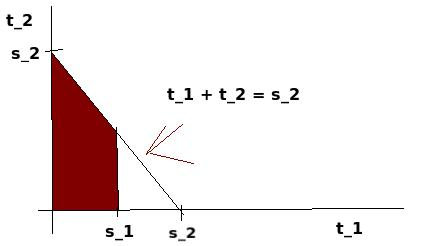
\includegraphics{4_8.jpeg}
    \begin{eqnarray*}
      P(S_1 \le s_1, S_2 \le s_2) 
        & = & P(T_1 \le S_1 , T_1 + T_2 \le S_2)\\
        & = & \int_0^{s_1} dt_1 \int_0^{s_2 - t_1} dt_2 f_{T_1, T_2}(t_1, t_2)\\
      f(s_1, s_2) 
        & = & \frac{\sigma}{\sigma s_2}\int_0^{s_2 - s_1} dt_2 f_{T_1, T_2}(s_1, t_2)\\
        & = & f_{T_1, T_2}(s_1, s_2 - s_1)\\
        & = & f_{T_1}(s_1)f_{T_2}(s_2 - s_1)\\
        & = & \lambda e^{-\lambda s_1} \lambda e^{-\lambda (s_2 - s_1)}\\
        & = & \lambda^2 e^{-\lambda s_2}
    \end{eqnarray*}
    Therefore,
    $$
      f(s_1, s_2) = 
        \begin{cases}
          \lambda^2 e^{-\lambda s_2} & \text{if } 0 \le s_1 \le s_2\\
          0 & \text{otherwise}
        \end{cases}
    $$
    $f_{s_2}(s) = \lambda^2 s_2 e^{-\lambda s_2}$ for $s_2 \ge 0$.\\
    Therefore,
    $$
      f_{S_1| S_2}(s_1 | s_2) = \frac{\lambda^2 e^{-\lambda s_2}}{\lambda^2 s_2 e^{-\lambda s_2}}
         = \frac{1}{s_2}
    $$
    give that $0 \le s_1 \le s_2$ and 0 otherwise.\\
    Therefore, given that if we know when the second bulb fails, the first 
    bulb can fails follow the uniform distribution between $0$ and $s_2$.

  \subsection*{Computing expectataions and probability by conditioning}
    \underline{Example}: Roll a die. Assume the number rolled is $N$.
      Then, continue rolling until you either match or exceed $N$.
      What is the expected number of additional rolls?\\
      This is geometric if we know $N$, so let's condition on the
      value of $N$.\\
      Let $X$ be the number of additional rolls.\\

      \begin{eqnarray*}
        E(X|N = n)
          & = & \frac{6}{7-n}\\
        E(X) 
          & = & \sum_{n = 1}^6 E(X|N = n) P(N = n)\\
          & = & \frac{1}{6}\sum_{n=1}^6 \frac{6}{7-n}\\
          & = & \sum_{n=1}^6 \frac{1}{7-n}\\
          & = & 1 + \frac{1}{2} + \frac{1}{3} + \ldots + \frac{1}{6}
      \end{eqnarray*}
    \underline{Example}: the number $N$ customers entering a store on a given 
      day is $Poisson(\lambda)$. Each of them buys something independent with
      probability $p$.\\
      Compute the probability that $k$ people buy something.\\

\section*{4/10}
  Let $N$ be the number of people entering the store. It follows Poisson($\lambda$)\\
  Each buys something with probability $p$, indepedently.\\
  Let $X$ be the number of people who buy something.\\
  Why should $X$ be Poisson? Approximate:\\
  Let $n$ be the population of the town\\
  Let $\epsilon$ be the probability that a person enteres the store.\\
  $\lambda = n\epsilon$.\\
  Let $N \approx Binomial(n, \epsilon)$.\\
  Let $X \approx Binomial(n, p\epsilon)$.\\
  \begin{eqnarray*}
    P(X=k) & = & \sum_{n = k}^{\infty} P(X = k | N = n)P(N=n)\\
      & = & \sum_{n = k}^{\infty} \binom{n}{k}p^k(1-p)^{n-k} \frac{\lambda^ne^{-\lambda}}{n!}\\
      & = & e^{-\lambda} \sum_{n = k}^{\infty}\frac{n!}{k!(n-k)!} p^k (1-p)^{n-k} \frac{\lambda^n}{n!}\\
      & = & \frac{e^{-\lambda}p^k \lambda^k}{k!} \sum_{n = k}^{\infty} 
        \frac{(1-p)^{n-k}\lambda^{n-k}}{(n-k)!}\\
      & = & \frac{e^{-\lambda}(p\lambda)^k}{k!}\sum_{l = 0}^{\infty}\frac{((1-p)\lambda)^l}{l!}\\
      & = & \frac{e^{-\lambda}(p\lambda)^k}{k!} e^{(1-p)\lambda}\\
      & = & \frac{e^{-p\lambda}(p\lambda)^k}{k!}
  \end{eqnarray*}
  Therefore, it is in fact, Poisson($p\lambda$).\\
  \underline{Example}: Toss a coin repeatedly with probability of getting heads $p$.\\
    What is the expected number of times need to get $k$ sucessive heads?\\
    (\underline{Note}: If you remove "successive", the answer is $\frac{k}{p}$)\\
    Let $N_k$ be the number of tosses required.\\
    Let's condition on $N_{k-1}$.\\
    \begin{eqnarray*}
      E[N_k | N_{k-1} = m] & = & 
        p(m+1) + (1-p)(m+1 + E(N_k))\\
        & = & pm + p + (1-p)m + 1-p + m_k (1 - p)\\
        & = & m+1 + m_k(1-p)\\
      m_k = E(N_k) & = & \sum_{m=k-1}^{\infty} E[N_k|N_{k-1}=m] P(N_{k-1} = m)\\
        & = & \sum_{m=k-1}^{\infty} [m+1 + m_k(1-p)] P(N_{k-1})\\
        & = & m_{k-1} + 1 + m_k(1-p)\\
        & = & \frac{1}{p} + \frac{m_{k-1}}{p}\\
      m_1 & = & \frac{1}{p}\\
      m_2 & = & \frac{1}{p} + \frac{1}{p^2}\\
      m_3 & = & \frac{1}{p} + \frac{1}{p^2} + \frac{1}{p^3}\\
      & \vdots &
    \end{eqnarray*}
    \begin{enumerate}
      \item $p(m+1)$ is the probability that you have heads on the $m+1$ try times
        its value.
      \item Otherwise, it's tails and however long it is to get it again
    \end{enumerate}
  \underline{Example}: Gambler's ruin\\
    We have a random walk on the integers.\\
    For a given spot, you have a probability of $p$ to walk one step forward.\\
    Otherwise, you walk one step backwards.\\
    What is your probability reaching $N$ before reaching $0$?\\
    Call this probability, $P_i$
    "One step conditioning",
    \begin{eqnarray*}
      P_0 & = & 0\\
      P_N & = & 1\\
      P_i & = & pP_{i+1} + (1-p)P_{i-1}\\
      P_{i+1} - P_{i} & = & \frac{1-p}{p} (P_i - P_{i-1})\\
      P_2 - P_1 & = & \frac{1-p}{p}(P_1 - P_0)\\
        & = & \frac{1-p}{p}P_1\\
      P_3 - P_2 & = & \left(\frac{1-p}{p}\right)^2(P_1)\\
      & \vdots&\\
      P_N - P_{N-1} & = & \left(\frac{1-p}{p}\right)^{N-1}P_1\\
      P_i & = & P_1\left(1 + \left(\frac{1-p}{p}\right)+ \left(\frac{1-p}{p}\right)^2+ \ldots+ \left(\frac{1-p}{p}\right)^N\right) 
    \end{eqnarray*}

\section*{4/13}
  \subsection*{Gambler's ruin}
    Every round, you either win a dollar with probability, $p$. otherwise,
    you lose a dollar.\\
    What is my probability that I will reach $N$ before I hit 0?\\
    Let $P_i = P($ reaching $N$ before reaching 0$)$.\\
    Let $X_1 = \begin{cases} 
      1 & \text{win a dollar on 1st round}\\
      -1 & \text{lose a dollar on 1st round}\\
    \end{cases}$\\
    Let 
    \begin{eqnarray*}
      P_i & = & P(\text{reach $N$ before reaching 0} | X_1 = 1)P(X_1 = 1) + 
        P(\text{reach $N$ before reaching 0} | X_1 = -1)P(X_1 = -1)\\
        & = & P_{i+1}p + P_{i-1}(1-p)
    \end{eqnarray*}
    This is a recurrence relation.\\\\
    \begin{eqnarray*}
      P_2 - P_1 & = & \frac{1 - p}{p} P_1\\
      P_3 - P_2 & = & \frac{1 - p}{p} (P_2 - P_1) = \left(\frac{1 - p}{p}\right)^2  P_1\\
      & \vdots &\\
      P_i - P_{i-1} & = & \left(\frac{1 - p}{p}\right)^{i-1} P_1 \text{ where }
      i = 1, \ldots, N\\
    \end{eqnarray*}
    We know that $P_0 = 0$ and $P_N = 1$.\\
    We also know that
    \begin{eqnarray*}
      P_i - P_1 & = & \left( \left(\frac{1-p}{p}\right) + \left(\frac{1-p}{p}\right)^2 + \ldots + \left(\frac{1-p}{p}\right)^{i-1}\right)P_1\\
      P_i & = & \left( 1+ \left(\frac{1-p}{p}\right) + \left(\frac{1-p}{p}\right)^2 + \ldots + \left(\frac{1-p}{p}\right)^{i-1}\right)P_1\\
      P_i & = & \frac{1 - \left(\frac{1-p}{p}\right)^i}{1 - \frac{1-p}{p}}P_1 \text{ where } p \not= \frac{1}{2}\\
      P_i & = & ip_1 \text{ where } p = \frac{1}{2}\\
    \end{eqnarray*}
    Let's use $P_N = 1$
    $$
      P_i = \begin{cases}
        \frac{1 - \left(\frac{1 - p}{p}\right)^i}{1 - \left(\frac{1 - p}{p}\right)^N} & p \not= \frac{1}{2}\\
        \frac{i}{N} & p = \frac{1}{2}
      \end{cases}
    $$
    Let $p = \frac{1}{2}$, $N = 10$, $i = 5$, $P_i = \frac{1}{2}$.\\
    Let $p = .6$, $N = 10$, $i = 5$, $P_i = .87$.\\
    Let $p = \frac{18}{38}$, $N = 1000$, $i = 900$, $P_i = 3 \cdot 10^{-5}$

    \noindent\underline{Best Strategy}: "Bold Play"\\
      You have amount, $x$ and want to get to $N$. The strategy is as follows:
      \begin{enumerate}
        \item Bet $x$ if $x \le \frac{N}{2}$
        \item Bet $N - x$ if $x \ge \frac{N}{2}$
      \end{enumerate}
      You can assume that $N = 1$.\\
      Let $P(X) = P(\text{get to $N$ before 0})$\\
      $$
        P(X) = \begin{cases}
          p \cdot P(2x) & x \in [0, \frac{1}{2}]\\
          p \cdot 1 + (1-p) \cdot P(2x - 1) & x \in [\frac{1}{2}, 1]
        \end{cases}
      $$
      We can compute by solving a linear system on $\frac{k}{2^n}$, where $k = 0, \ldots, 2^n$\\
      Let $n = 1$. $p = P\left(\frac{1}{2}\right)$\\
      Let $n = 2$. $p^2 = P\left(\frac{1}{4}\right)$, $P\left(\frac{3}{4}\right) = p + (1-p)p$\\
      Let $n = 3$. $p^3 = P\left(\frac{1}{4}\right)$, 
        $P\left(\frac{3}{8}\right) = pP\left(\frac{3}{4}\right) = p^2 + p^2(1-p)$,
        $P\left(\frac{5}{8}\right) = p +  p^2(1-p)$,
        $P\left(\frac{7}{8}\right) = p +  p(1-p) + p(1-p)^2$.\\\\
      $P(.9) = .88, \text{ for } p = \frac{12}{38}$\\
      $P(X) = x$ when $p = \frac{1}{2}$.\\
    
    \noindent\underline{Remark}: Look at the function, $P(x)$. Graph it. It's nowhere
      differentiable, but continuous in its domain. It's highly irregular. It's
      strictly increasing. You can even solve the recurrence. Let $P(x) = P(Y \le x)$.\\
      $$
        Y = \sum_{j = 1}^{\infty} D_j \frac{1}{2^j} \text{ where $D_j$ is the $j$th digit}
      $$
      $$
        P(D_j = 1) = p
      $$
      $$
        P(D_j = 0) = 1- p
      $$

    \noindent\underline{Example}: Assume that you keep flipping a fair coin until you get
      heads. Each time you flip tails, roll a die, and collect as many dollars as number
      shown on the die.\\
      Let $Y$ be the amount you win. Calculate $EY$, $Var(Y)$.\\
      We have a sum of iid with random number of terms.\\
      Let $X_1, X_2, \ldots$ be iid with $EX_1 = \mu$ and $Var(X_1) = \sigma^2$\\
      Let $N$ be independent of all $X$'s.\\
      Take 
      $$
        S = \sum_{k = 1}^N X_i
      $$
      Compute $ES$, $Var(S)$.

\section*{4/14}
  Sums with random number of terms.
  $$
    X_1, X_2, \ldots
  $$
  Say the terms are iid.\\
  Let $N$ be the another (nonnegative integer) random variable, 
  independent of $X_i$.\\
  We want to find out $E(S)$ and $Var(S)$ if $S = \sum_{i = 0}^NX_i$\\
  $$
    E[S| N = n] = nE(X_1)
  $$
  Then,
  \begin{eqnarray*}
    E[S] & = & \sum_{n = 0}^{\infty}nE(X_1)P(N=n)\\
      & = & E(X_1)E(N)
  \end{eqnarray*}
  Now, the variance
  \begin{eqnarray*}
    E(S^2) & = & \sum_{n = 0}^{\infty} E[S^2 | N = n]P(N = n)\\
      & = & \sum_{n = 0}^{\infty} E((\sum_{i = 1}^n X_i)^2)P(N= n)\\
      & = & \sum_{n = 0}^{\infty} ((Var(\sum_{i = 1}^n X_i))+(E(\sum_{i = 1}^nX_i))^2)P(N=n)\\
      & = & \sum_{n = 0}^{\infty} [nVar(X_1) + n^2(EX_1)^2]P(N = n)\\
      & = & Var(X_1)E(N) + E(X_1)^2 E(N^2)\\
  \end{eqnarray*}
  Therefore,
  \begin{eqnarray*}
    Var(S) & = & E(S^2) - (ES)^2\\
      & = & Var(X_1)E(N) + (EX_1)^2E(N^2) - (EX_1)^2(EN)^2\\
      & = & Var(X_1)E(N) + (EX_1)^2Var(N)
  \end{eqnarray*}

  \noindent\underline{Example}: Toss a fair coin until 1st heads. Each time
     you toss tails, roll a die, collect as many dollar as the number on the 
     die. Let $Y$ be your total winnings. Compute $EY$ and $Var(Y)$.\\

     $$
      EX_1 = \frac{7}{2}
     $$
     $$
      E(X_1^2) = \frac{1}{6}(1^2 + \ldots + 6^2)
     $$
     $$
      Var(X_1) = \ldots = \frac{35}{12}
     $$
     Let $N$ be the number of failures before successs, which is a geometric
     random variable - 1.\\
     $EN = 2 - 1 = 1$.\\
     $Var(N) = \frac{\frac{1}{2}}{\left(1- \frac{1}{2}\right)^2} = 2$
     Plug in and get $Var(Y) = \frac{59}{12}$.

  \subsection*{Markov Chains}
    Consider the following experiments with a book:
    \begin{enumerate}
      \item Pick letters at random and do it random in sucession.
      \item Start by a random letter. Next, pick a letter at random such that
        it succeeds the previous letter, and repeat.
      \item Start the same way. Next, pick a letter at random from letters
        which are at or after, in alphabetical order, the position of the
        previous letter.
    \end{enumerate}
    \begin{definition}
      Let $X_0, X_1, \ldots$ be a sequence of random variables. This is 
      called a \underline{Markov Chain} if the distribution of $X_{n+1}$
      (where $n = 0, 1, \ldots$ only depends on the value of $X_n$.
    \end{definition}
    \underline{Note}: We will often assume that the possible values of $X_n$ be 
      non-negative integers. This means that $X_n$ has countably many values.

    \noindent The information about the process is given by the 
      \underline{transition probabilities},
      $$
        P_{ij} = P(X_{n+1} = j | X_n = i)
      $$
      "Given at stage $n$, we are in state $i$, we move to state $j$ in
      the next state."\\
      \underline{Note}: $P_{ij}$ does not depend on $n$.\\
      \underline{Note}: $P_{ij}\ge 0$, $\sum_j P_{ij} = 1$.


\section*{4/15}
  \underline{Example}:
    Have a book. Choose a random letter. Then, at each step, either
    \begin{enumerate}
      \item Pick another random letter (Markov)
      \item choose a random occurence of the person's letter, then 
        pick next letter (next letter to last is the 1st letter).
        (is also Markov)
      \item Choose a random occurence of the last two letters, in 
        order, then pick next letter (not Markov, but becomes
        Markov if you keep track of two letters)
      \item Choose a random occurences of all previously chosen
        letters, in order, then pick next letter (not Markov)
      \item In step $n$, choose a random letter with probability
        $\frac{1}{n}$ and do $(2)$ with probability, $1 - 
        \frac{1}{n}$
    \end{enumerate}
    Let $X_0, X_1, \ldots$ be a sequence of discrete random 
    variables with random variables with values, most often, $0, 1, 
    2,\ldots$. The information about the Markov chain is given by
    the \underline{transition probabilities},
    $$
      P_{ij} = P(X_{n+1} = j | X_n = i)
    $$
    There is also a \underline{transition matrix} represented by
      $\left[
        \begin{array}{c c c c} 
          P_{11} & P_{12} & P_{13} & \ldots\\
          P_{21} & P_{22} & P_{23} & \ldots\\
          &\vdots & &\\
        \end{array}
      \right]$.\\
    This is also known as a stochastic matrix. Row sums are 1.\\

    \noindent\underline{Example}: The random moves to the right (by 1)
      with probability, $p$, and to the left with probability $1-p$,
      except when it at 0 or 4. These two states are \underline{absorbing}
      once there, the walker does not move.
      $$
        P = \left[
        \begin{array}{c c c c c} 
          1 & 0 & 0 & 0 & 0 \\
          1 - p & 0 & p & 0 & 0\\
          0 & 1 - p & 0 & p & 0\\
          0 & 0 & 1-p & 0 & p\\
          0 & 0 & 0 & 0 & 1
        \end{array}
      \right]
      $$

    \noindent\underline{Example}: Same as the previous example except that 0 or
    4 are \underline{reflecting}. From 0, always move to 1. From 4, always move 
    to 3.
    $$
        P = \left[
        \begin{array}{c c c c c} 
          0 & 1 & 0 & 0 & 0 \\
          1 - p & 0 & p & 0 & 0\\
          0 & 1 - p & 0 & p & 0\\
          0 & 0 & 1-p & 0 & p\\
          0 & 0 & 0 & 1 & 0
        \end{array}
      \right]
      $$

    \noindent\underline{Example}: A general random walk on a graph, 
      walker moves to a randomly chosen neighbor. I have a graph with
      4 nodes, $a, b, c, d$. Here's an adjacency matrix of their movements.
      $$
      \left[
        \begin{array}{c c c c} 
          0 & 1 & 0 & 1\\
          1 & 0 & 1 & 1\\
          0 & 1 & 0 & 1 \\
          1 & 1 & 1 & 0 
        \end{array}
      \right]
      $$
      It has the following transition matrix
      $$
      P = \left[
        \begin{array}{c c c c} 
          0 & \frac{1}{2} & 0 & \frac{1}{2}\\
          \frac{1}{3} & 0 & \frac{1}{3} & \frac{1}{3}\\
          0 & \frac{1}{2} & 0 & \frac{1}{2} \\
          \frac{1}{3} & \frac{1}{3} & \frac{1}{3} & 0 
        \end{array}
      \right]
      $$

    \noindent\underline{Example}: I have a graph with two nodes.
      Node 0 transitions to node 0 with probability $\alpha$\\
      Node 0 transitions to node 1 with probability $1-\alpha$\\
      Node 1 transitions to node 1 with probability $\beta$\\
      Node 1 transitions to node 0 with probability $1 - \beta$\\
      Here is the transition matrix
      $$
        P = \left[ 
          \begin{array}{c c} 
            \alpha & 1 - \alpha\\
            1 - \beta & \beta\\
          \end{array}
        \right]
      $$

    \noindent\underline{Example}: "Changeover" Keep track of two toss sequences
      in an infinite sequence of coin tosses with probability $p$ of heads.
      $$
        \left[ 
          \begin{array}{c c c c c} 
            States & HH & HT & TH & TT\\
            HH & p & 1 - p & 0 & 0\\
            HT & 0 & 0 & p & 1 - p\\
            TH & p & 1 - p & 0 & 0\\
            TT & 0 & 0 & p & 1 - p\\
          \end{array}
        \right]
      $$
      The horizontal axis is the current flip and the previous flip. The 
      vertical axis is the previous two flips.\\

    \noindent\underline{Example}: Random walk on $\mathbb{Z}$.\\

    \noindent\underline{Example}: Birth-death chain. Let's say my population
    is $X$. Assume it absorbs at 0. We have a probability $p_x$ be the 
    probability of birth and $q_x$ be the probability of death and $r_x$
    be the probability of death and birth. The transition matrix is pretty much
    a diagonal.

\section*{4/17(discussion)}
  Prove
  $$
    \lim_{n \to \infty} e^{-n} \sum_{n \to \infty}\frac{n^k}{k!} = \frac{1}{2}
  $$
  We're going to use Central limit theorem. to use cental limit theorem,
  you need to realize
  $$
    X_n = \sum_{i = 1}^n Y_i
  $$
  The former is Poisson($n$), while $Y_i$ is Poisson($1$).\\
  \underline{Fact}: $A$ and $B$ are Poisson with parameters $a$ and $b$ 
    respectively, then $A+B$ is Poisson with Poisson$(a+b)$.\\
  \begin{proof}
    \begin{eqnarray*}
      P(A+B \le n) & = & \sum_{l = 0}^n P(A = l, B= n-l)\\
        & = & \sum_{l = 0}^n P(A = l)P(B= n-l) \text{ (Remember, iid)}\\
        & = & \sum_{l = 0}^n e^{-a}\frac{a^l}{l!} \cdot e^{-b}\frac{b^{n-l}}{(n-l)!}\\
        & = & e^{-a - b}\frac{(a+b)^n}{n!}\\
    \end{eqnarray*}
  \end{proof}
  Therefore, $EX_n = n$ and $Var(X_n) = n$ since $EY_i = 1$ and $Var(Y_i) = 
  1$.\\
  By the central limit theorem
  $$
    P\left(\frac{X_n -n}{\sqrt{n}} \le 0 \right) \to \Phi(0) = \frac{1}{2}
  $$

\subsection*{3.41}
  Let $X$ be a random variable describing total time to exit
  \underline{Idea}: Define random variable, 
  $$
    I = 
    \begin{cases}
      1 & \text{left}\\
      0 & \text{right}\\
    \end{cases}
  $$
  \begin{eqnarray*}
    E(x) & = & E(E(X |I))\\
      & = & E(X | I = 0)P(I = 0) + E(X |I = 1)P(I = 1)\\
      & = & \sum_{x}xP(X = x | I = 0)P(I = 0) + \sum_{x}xP(X = x | I = 1)P(I = 1)\\
      & = & \sum_{x}x\frac{P(X = x, I = 0)}{P(I = 0)}P(I = 0) + \sum_{x}x\frac{P(X = x, I = 1)}{P(I = 1)}P(I = 1)\\
      & = & \sum_{x}xP(X = x, I = 0) + \sum_{x}xP(X = x, I = 1)\\
  \end{eqnarray*}

\section*{4/20}
  \subsection*{Markov Chain}
    Determined by
    \begin{itemize}
      \item \underline{state space}: a countable set, often represented
        by positive numbers.
      \item \underline{transition probabilities}
        $$
          P_{ij} = P(X_{n+1} = j | X_n = i)
        $$
        which satisfy $P_{ij} \ge 0$, $\sum_j P_{ij}, \forall i$
      \item \underline{initial state}
    \end{itemize}
    Graphically, one often represents a Markov Chain like this:\\
    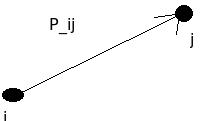
\includegraphics{4_20.jpeg}\\
    $$
      P_{ij}^n = P(X_n = j | X_0 = i) (= P(X_{n+m} = j | X_m = i))
    $$
    $$
      P_{ij}^1 = P{ij}
    $$
    This is called the \emph{n-step probabilities}.\\
    \begin{eqnarray*}
      P_{ij}^{n+m} & = & P(X_{n+m} = j | X_0 = i)\\
        & = & \sum_k P(X_{n+m} = j, X_n = k | X_0 = i) \text{ ($X_0 =i$ isn't really a condition. It's just the starting state)}\\
        & = & P(X_{n+m} = j | X_n= k)P(X_n = k | X_0 = i) \\
        & = & P(X_{m} = j | X_0= k)P(X_n = k | X_0 = i) \text{ (doesn't matter how you got there.)}\\
        & = & \sum_k P_{kj}^m P_{ik}^n \\
    \end{eqnarray*}
    Let $P^{(n)}$ be the matrix, $P_{ij}^n$
    \begin{eqnarray*}
      P^{(m+n)}  & = & P^{(n)}P^{(m)} \\
      P^{(n)} & = & P^{(1)}P^{(1)} \ldots P^{(1)}\\
        & = & P^n
    \end{eqnarray*}
    Conclusion: Computing $n$-step transition probability is the same as
    computing powers of $P$.\\

    \noindent \underline{Example}: Two state Markov Chain defined by
    $$
      P = \left[\begin{array}{c c} \alpha & 1 - \alpha\\ \beta & 1 - \beta
        \end{array}\right]
    $$
    Then,
    $$
      P^2 = \left[\begin{array}{c c} \alpha^2 + (1 - \alpha)\beta 
        & \alpha(1 - \alpha) + (1 -\alpha) (1 - \beta)\\ 
        \alpha\beta + (1 - \beta)\beta 
        & \beta(1 - \alpha) + (1 - \beta)^2
        \end{array}\right]
    $$
    Assume now, that initial distribution is given by
    $$
      \alpha_i = P(X_0 = i), \forall i, (\sum_i \alpha_i = 1, \alpha_i \ge 0)
    $$
    \begin{eqnarray*}
      P(X_n = j) & = & \sum_i P(X_n = j | X_0 = i)P(X_0 = i)\\
        & = & \sum_i \alpha_i P_{ij}^n\\
    \end{eqnarray*}
    The row of probabilities is given by
    $$
      P(X_n = i) = [\alpha_0, \alpha_1, \ldots ]P^n
    $$

    \noindent\underline{Example}: Random walk on the graph below:\\
    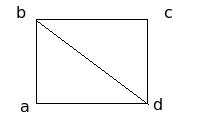
\includegraphics{4_20_2.jpeg}\\
    Choose starting point at random. What is the probability that a random
    walk is at $a$ after 2 steps. At each vertex, you are equally likely to
    choose any of the edges it is connected to.\\
    $$
      P = \left[\begin{array}{c c c c}
        0 &  \frac{1}{2} & 0 & \frac{1}{2}\\
        \frac{1}{3} & 0 & \frac{1}{3} & \frac{1}{3}\\
        0 & \frac{1}{2} & 0 & \frac{1}{2}\\
        \frac{1}{3} & \frac{1}{3} & \frac{1}{3} & 0
        \end{array}\right]
    $$
    $$
      \left[\begin{array}{c c c c} \frac{1}{4} & \frac{1}{4} & \frac{1}{4}
        & \frac{1}{4}\end{array}\right] P^2 = \left[\begin{array}{c c c c} P(X_2 = 1) & P(X_2 = 2) & P(X_2 = 3) & P(X_2 = 4)\end{array}\right]
    $$
  \subsection*{Classification of states}
    \begin{itemize}
      \item We say that a state $j$ is \underline{accessible from state $i$}
        if $P_{ij}^n > 0$ for some $n > 0$. (there is a possibility of 
        reaching $j$ from $i$ in any number of steps).
      \item If $i$ is accessible from $j$, and $j$ is accessible from $i$,
        then we say that $i$ and $j$ are \underline{coummunicate}, $i 
        \leftrightarrow j$
      \item "$\leftrightarrow$" is an \underline{equivalence relation}.
        \begin{itemize}
          \item $i \leftrightarrow i$
          \item $i \leftrightarrow j \Rightarrow j \leftrightarrow i$
          \item $i \leftrightarrow j$ and $j \leftrightarrow k \Rightarrow i \leftrightarrow k$
        \end{itemize}
    \end{itemize}
    \underline{Example}:\\ 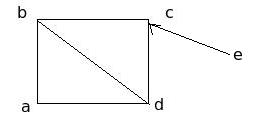
\includegraphics{4_20_3.jpeg}\\
    Any state, $a, b, c, d$ is accessible from $e$, but $e$ is not accessible
    from $a, b, c, d$.\\
    $e$ is accessible from $e$ by definition.\\

\section*{4/24}
  If $j$ is not accessible from $i$, then
  $P_{ij}^n = 0$ $\forall n$.\\
  \begin{eqnarray*}
    P(\text{ ever visit } j | X_0 = i)
    & = & P(\bigcup_{n = 0}^{\infty} \{ X_n = j\} | X_0 = i)\\
    & \le & \sum_{n = 0}^{\infty}P(X_n = j | X_0 = i) = 0
  \end{eqnarray*}
  Also, note that accessibility, etc..., the site of elements in $P$ does not
  matter, all that matters is which are positive and which 0.\\
  If the chain has $M$ states, then $j$ is accessible from $i$ iff for some
  $n \le M(P + P^2 + \ldots + P^m)_{ij} > 0$\\
  The communication relation "$\leftrightarrow$" is an equivalence relation
  \begin{enumerate}
    \item $i \leftrightarrow i$
    \item $i \leftrightarrow j$ implies $j \leftrightarrow i$
    \item $i \leftrightarrow j$ and $j \leftrightarrow i$ implies $i 
      \leftrightarrow k$
  \end{enumerate}
  To prove (3), it is enough to prove
  $$
    (i \rightarrow j) \text{ and } (j \rightarrow k) \text{ implies }
    i \rightarrow k
  $$
  This holds because
  $\exists n$ so that $P_{ij}^n > 0$\\
  $\exists n$ so that $P_{ij}^m > 0$\\
  Then, $P_{ik}^{m + n} > 0$\\
  This relation divides states into \underline{classes} within a class, all
  states communicate to each other. This chain is \underline{irreducible}
  if there is only one class. (If we have $m$ states, that means all entries of $I + P
  + \ldots + P^M$ are positive)

  \noindent\underline{Example}:
    $$
      P = \left[\begin{array}{c c c}
        \frac{1}{2} & \frac{1}{2} & 0\\
        \frac{1}{2} & \frac{1}{4} & \frac{1}{4}\\
        0 & \frac{1}{3} & \frac{2}{3}
      \end{array}\right]
    $$
    As we can see, $0 \leftrightarrow 1$, $1 \leftrightarrow2$, so irreducible.

  \noindent\underline{Example}:
    $$
      P = \left[\begin{array}{c c c c}
        \frac{1}{2} & \frac{1}{2} & 0 & 0\\
        \frac{1}{2} & \frac{1}{2} & 0 & 0\\
        0 & 0 & 0 & 1\\
      \end{array}\right]
    $$

  For any state $i$, denote
  $$
    f_i = P(\text{ ever reenter } i | X_0 = i)
  $$
  We call a state \underline{recurrent} if $f_i = 1$.\\
  We call a state \underline{transient} if $f_i < 1$.\\

  \noindent From previous example, $f_2 = \frac{1}{4}$, so 2 is 
    transient.\\
    $f_3 = 1$, so 3 is recurrent.
    $f_0 = 1$ because the only possibility that it isn't recurrent
      is if we go to state $1$ and stay there forever. As $n \to
      \infty$, $\left(\frac{1}{2}\right)^n = 0$, so the probability
      of it staying at 1 is 0. Therefore, it's 1.\\
    $f_1 = 1$ by similar logic as above.\\
    Therefore, $f_0$ and $f_1$ are recurrent states.\\

  The Markov Chain visits a recurrent state infinitely many times, or
  not at all. (starting from an arbitrary state).\\
  On the other hand,
  $$
    P(\text{reenter $i$ exactly $n$ times} | X_0 = i) = f_i^{n-1}(1 - f_i)
  $$
  Therefore, the number of times spent at $i$ is a geometric random variable
  with success(which is never returning in this case) probability of
  $1 - f_i$, so our expectation is $\frac{1}{1-f_i}$.

\section*{4/27}
  $f_i = P($ ever reenter $i | X_0 = i)$\\
  The state $i$ is \underline{recurrent} if $f_i = 1$.\\
  The state $i$ is \underline{transient} if $f_i < 1$.\\
  $P($ visit $i$ $n$ times $| X_0 = i) = f_i^{n-1}(1 - f_i)$\\
  $$
    E(\text{number of visits to } i | X_0 = i) = \frac{1}{1 - f_i}
  $$
  $$
    E(\text{number of visits to } i | X_0 = i) = E(\sum_{n = 0}^{\infty} I_n | X_0 = i)
  $$
  where $I_n = I\{X_n = i\}$, $n = 0, 1, 2, \ldots$\\
  \begin{eqnarray*}
    I_n & = & \sum_{n = 0}^{\infty}P(X_n = i | X_0 = i)\\
      & = & \sum_{n = 0}^{\infty}P_{ii}^n\\
  \end{eqnarray*}
  \begin{theorem}
    1 is recurrent $\Leftrightarrow$  $\sum_{n = 1}^{\infty}P_{ii}^n = \infty$
  \end{theorem}
  If a Markov chain only has finitely many states, then there must be at 
  least one recurrent state. Why?\\
  If all states are transient, then all the states will be visited only finitely
  many times. That is impossible. \\
  \begin{proposition}
    If $i$ is recurrent, and $i \leftrightarrow$ j, then also, $j$ is recurrent.
    If the chain is irreducible, then either all states are recurrent or all
    transient.
  \end{proposition}
  \begin{proof}
    $P_{ij}^k > 0, P_{ji}^m > 0$ for some $k,m$.\\
    For any $n \ge 0$:
    $$
      P_{ij}^{m + n + k} \ge P_{ji}^m P_{ii}^n P_{ij}^k
    $$
    If a state is recurrent, then $f_i = 1$. \\
    Then, $E(\text{number of visits to } i | X_0 = i) = \frac{1}{1 - f_i} = \infty$.\\
    If $\sum_{n = 0}^{\infty} P_{ii} = \infty$, then 
    $\sum_{n = 0}^{\infty} P_{jj}^{m+n+k}=\infty$, so
    $\sum_{l = 0}^{\infty} P_{jj}^{l} = \infty$.\\
    If $i$ is recurrent, then so is $j$.
  \end{proof}

  \noindent\underline{Example}:
  $$
    P = \left[
      \begin{array}{c c c c}
        0 & 0 & \frac{1}{2} & \frac{1}{2}\\
        1 & 0 & 0 & 0\\
        0 & 1 & 0 & 0\\
        0 & 1 & 0 & 0\\
      \end{array}
      \right]
  $$
  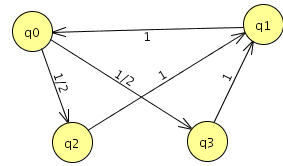
\includegraphics{Ex1_4_27.png}\\
  As we can see every element can reach each other, so the chain is 
  irreducible. We can also see that state 0 whether it chooses to
  go to state 2 and 3 will end up at state 1 and back to state 0.
  Therefore, it is recurrent and the entire thing is also recurrent.\\

  \noindent\underline{Example}:
    $$
      P = \left[
        \begin{array}{c c c c c c}
          0 & 1 & 0 & 0 & 0 & 0\\
          4 & 6 & 0 & 0 & 0 & 0\\
          3 & 0 & 4 & 2 & 1 & 0\\
          0 & 0 & 0 & 3 & 7 & 0\\
          0 & 0 & 0 & 5 & 0 & 5\\
          0 & 0 & 0 & 3 & 0 & 2\\
        \end{array}
      \right]
    $$
    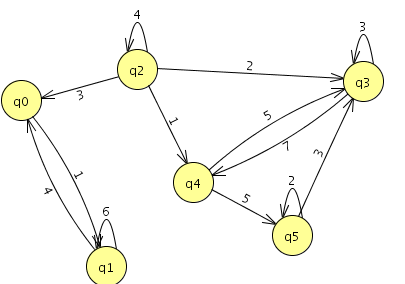
\includegraphics{Ex2_4_27.png}\\
    As we can see, nothing can reach 2 besides 2 itself. Therefore, 2 is
    in a group of its own. 0 and 1 can reach other and nothing else, so it
    is in a group of its own. 3, 4, and 5 can reach each other.\\
    As we can see, 2 can only reach itself sometimes. Therefore, $j_2 < 1$ 
    making it transient.\\
    When we are at state 1 and choose to go to 0, it will always come back to 1.
    Also, state 1 can choose to stay. Therefore, $j_1 = 1$, which then
    means that $j_0 = 1$ making both of them recurrent.\\
    We can also see that $\{3, 4, 5\}$ is recurrent.\\

  \noindent\underline{Example}:
    Simple random walk on $\mathbb{Z}$. When $p = \frac{1}{2}$, this is
    a simple symmetric random walk.\\
    Simple random walk on $\mathbb{Z}^2$.\\
    Simple random walk on $\mathbb{Z}^3$.\\
    Higher dimensions makes for lower probability to return to origin.\\
    In the 1 dimension case, 
    $$
      P_{00}^{2n - 1} = 0 \text{ (because if you walk out $n$ steps, 
        you need to walk back $n$ steps)}
    $$
    $$
      P_{00}^{2n} = \binom{2n}{n}p^n(1 - p)^n \text{($n$ steps to the 
        left and $n$ steps to the right. Pick $n$ steps out of $2n$ 
        steps to be left.)}
    $$
    Stirling's formula:
    $$
      n! \approx n^ne^{-n} \sqrt{2\pi n}
    $$
    So, according to Stirling's formula,
    \begin{eqnarray*}
      \binom{2n}{n} & = & \frac{(2n)!}{(n!)^2}\\
        & = & \frac{(2n)^{2n}e^{-2n}\sqrt{2\pi2n}}{n^{2n} e^{-2n} 2\pi n}\\
        & = & \frac{2^{2n}}{n\pi}
    \end{eqnarray*}



\section*{4/29}
  \subsection*{Continued from last time}
    \begin{eqnarray*}
      P_{00}^{2n - 1} & = & 0\\
      P_{00}^{2n} & = & \binom{2n}{n} p^n (1 - p)^n\\
        & \approx & \frac{2^{2n}}{\sqrt{n\pi}} p^n (1 - p)^n\\
        & = & \frac{1}{\sqrt{n\pi}} (4p(1-p))^n
    \end{eqnarray*}
    When $p = \frac{1}{2}$, $P_{00}^{2n} \approx 
      \frac{1}{\sqrt{n\pi}}$, $\sum_{n = 0}^{\infty} P_{00}^{2n} = 
      \infty$, so random walk is continuous.\\
    When $p \not= \frac{1}{2}$ , $P_{00}^{2n} \approx 
      \frac{1}{\sqrt{n\pi}}$, $\sum_{n = 0}^{\infty} P_{00}^{2n} <
      \infty$, so random walk is transient.\\
    Question: What is the $f_0 = P($ ever reenter 0 $| X_0 = 0)$?\\
    Gambler's ruin!\\
    Recall that
    $$
      P(\text{reach $N$ before 0} | S_0^{(1)} = 1) = 
      \begin{cases}
        \frac{1}{N} & p = \frac{1}{2}\\
        \frac{1 - \frac{1-p}{p}}{1 - \left(\frac{1 - p}{p}\right)^N}
        & \text{ otherwise}
      \end{cases}
    $$
    Also, that $P(\text{reach 0 before $N$ }| S_0^{(1)} = 1) = 
    1 - P(\text{reach $N$ before 0 }| S_0^{(1)} = 1)$.\\
    Let's send $N \to \infty$,
    $$
      P(\text{ever reach 0}| S_n^{(1)} = 1) =
      \begin{cases}
        1 & p = \frac{1}{2}\\
        1 & p < \frac{1}{2}\\
        \frac{1-p}{p} & p > \frac{1}{2}\\
      \end{cases}
    $$
    Assume that $p > \frac{1}{2}$. Then,
    \begin{eqnarray*}
      f_0 & = & P(\text{1st jump to 1 and it returns eventually}) +
      P(\text{1st jump to -1 and it returns eventually})\\
      & = & p\frac{1-p}{p} + (1-p)1 \\
      & = & 2(1-p)\\
    \end{eqnarray*}

  \subsection*{2 dimensional case}
    Drunk at Chicago problem. Drunk goes wandering around Chicago.
    What is the probability that the drunk comes back home?\\
    Let $S_n^{(2)}$ be the sequence of random walk.\\
    Let $k$ be the number of times walk moves in the $x$-direction.
    \begin{eqnarray*}
      P(\text{back at home(0,0) in $2n$ steps})
      & = & \sum_{k = 0}^n \binom{2n}{2k} \frac{1}{2^{2n}} 
        P(S_{2k}^{(1)} = 0) P(S_{2(n-k)}^{(1)} = 0)\\
    \end{eqnarray*}
    With overwhelming probability, $k \approx \frac{n}{2}$.\\
    Then,
    \begin{eqnarray*}
      P(S_{2k}^{(1)} = 0) & \approx & \frac{1}{\sqrt{n}}\\
      P(S_{2(n - k)}^{(1)} = 0) & \approx & \frac{1}{\sqrt{n}}\\
      P(\text{back at home(0,0) in $2n$ steps})
        & \approx & \frac{1}{n} \sum_{k = 0}^n \binom{2n}{2k} 
          \frac{1}{2^{2n}} \\
        & \approx & \frac{1}{n}\\
    P(\text{even number of steps in horizontal direction}) &\to& 
      \frac{1}{2}\\
      \sum_{n = 0}^{\infty}P(\text{back to (0,0) n(2n) step}) &=& 
      \infty
    \end{eqnarray*}
    So, the chain is still recurrent. In fact,
    \begin{eqnarray*}
      P(\text{back to 0 in $2n$ steps})
      & = & P(S_{2n}^{(1)} = 0)^2\\
    \end{eqnarray*}

  \subsection*{Random walk in 2 dimension with diagonals}
    Different random walk, but now that different. Rotate the
    lattice.\\
    As the two coordinates evolve independently.

\section*{5/1}
  \subsection*{Random walk in 3 dimensions}
    Squirrels walk around in a 3 dimensional maze. In this walk, you will walk
    $2k$ times in the z direction. Otherwise, it's running around in the x and
    y direction.\\

    It has $\frac{1}{3}$ probability of moving in the z-direction. In those $2k$ 
    steps, it has a probability, $P(S_{2k}^1 = 0)$ to come back to 0 in the 
    z-direction. \\

    \begin{eqnarray*}
      P(S_{2n}^{3} = 0) & = & \sum_{k = n}^n \binom{2n}{2k} 
        \left(\frac{1}{3}\right)^{2k} \left(\frac{2}{3}\right)^{2(n-k)} 
        P(S_{2k}^1 = 0)P(S_{2(n-k)}^{(2)} =0 )\\
      & \approx & \sum_{k = 0}^n \binom{2n}{2k} \left(\frac{1}{3}\right)^{2k} 
      \left(\frac{2}{3}\right)^{2(n-k)} \frac{1}{\sqrt{n}} \frac{1}{n}\\
      & = & \frac{1}{n^{3/2}}P(\text{ random walk makes even number of 
        steps in z direction})\\
      & \approx & \frac{1}{n^{3/2}} \frac{1}{2} \text{ (solve the binomial as $n \to \infty$)}\\
      \sum_n P(S_{2n}^{3} = 0) & < & \infty \text{ (so, the 3d random walk is transient)}\\
    \end{eqnarray*}
    Another way:
    \begin{eqnarray*}
      f_0 & = & \text{ probability of return to 0}\\
      \frac{1}{1 - f_0} & = & \sum_{n = 0}^{\infty} (P_{2n}^{(3)} = 0)\\
      & = & 1 + \frac{1}{6} + \ldots\\
      & = & \frac{1}{(2\pi)^3} \int_{(-\pi, \pi)^3} \frac{\,dx\,dy\,dz}{
        1 - \frac{1}{3}(\cos(x) + \cos(y) + \cos(z))} 
        \text{ (take an analysis course for why this is)}\\
    \end{eqnarray*}
    Aside, 
    Let $X = Binomial(n,p)$ random variables.\\
    $$
      p_n = P(X\text{ is even}) = \frac{1}{2}
    $$
    Why?
    \begin{eqnarray*}
      p_0 & = & 1\\
      p_{n + 1} & = & p_n (1 - p) + (1 - p_n) p\\
        & = & p + p_n (1 - 2p)\\
    \end{eqnarray*}
    Since we know it's $\frac{1}{2}$,
    $$
      p_n = \frac{1}{2} + c (1 - 2p)^n 
    $$
    $$
      1 = \frac{1}{2} + c, c = \frac{1}{2}
    $$
    So,
    $$
      p_n = \frac{1}{2} + \frac{1}{2} (1 - 2p)^n
    $$
    Plug this is all into the stuff and we get
    $$
      f_0 \approx .3405
    $$
    \underline{Remark}: A Markov chain can never leave a recurrent class, which is
    therefore often called \underline{closed}. 
    \begin{proof}
      Let $C$ be a recurrent class, $i \in C$ and $j \not\in C$. We need to show that
      $p_{ij} = 0$.\\

      Assume not, $p_{ij} > 0$. As $j$ does not communicate with $i$, the chain
      never reaches $i$ from $j$ ($i$ is not accessible from $j$).\\

      If the chain starts at $i$, it returns to there infinitely many times, so it
      eventually jumps to $j$ and never returns. CONTRADICTION!
    \end{proof}

  \subsection*{Branching processes}
    Unlike random walks problem, it has no spatial constraints.\\

    Consider a population of individuals which evolves according to the following
    rule: Each individual generation, $n$ produces a random number of 
    offsprings in the next generation independently from other individuals.\\

    $$
      P_i = P(\text{ number of offspring} = i)
    $$
    $i = 0, 1, 2, \ldots$\\
    
    Problem introduced by F. Galton (late 1800s). \\

    We will start with a single individual and they will produce offsprings.
    The graph of this structure is called a "Family tree".\\

    Let $X_n$ be the number of individuals in generation $n$ and $p_i$ be
    a probability mass function of the number of offsprings individual $i$
    will produce.
    \underline{Notes}:
    \begin{enumerate}
      \item If $X_n$ reaches 0, it's an absorbing state.
      \item $P(X_{n+1} = 0 | X_n = k) > 0$ provided $p_0^k > 0$
      \item Therefore, all states other than 0 are transient.
    \end{enumerate}
    \begin{eqnarray*}
      P(X_{n+1} = i | X_n = k) & = & P(S_1 + S_2 + \ldots + S_k = i)\\
    \end{eqnarray*}

\section*{5/4}
  \subsection*{Branching Process}
    Given $X_n = l$, $X_{n+1} = S_1 + \ldots + S_l$ where $S_i$ are
    iid with probability mass function given by $P_k$.\\
    Let $\pi_0$ be the probability that the process goes extinct and
    $P(X_n = 0)$ the population is extinct by time $n$.
    $\pi_0 = P(X_n = 0$ for some $n) = \lim_{n \to \infty} P(X_n = 0)$
    Compute $M_n = E(X_n)$ and $V_n = Var(X_n)$
    Using the equation above, 
    $$
      M_{n+1} = M_n\mu
    $$ and 
    $$
      V_{n+1} = M_n \sigma^2 + V_n\mu^2
    $$
    where $\mu = \sum_{k = 0}^{\infty} kP_k = EX_1$, $\sigma^2 =
    Var(X_1)$, $M_0 = 1$, and $V_0 = 0$. If we solve the recurrence,
    $$
      M_n = \mu^n
    $$
    Then,
    In conclusion, $P(X_n \ge 1) \le EX_n = \mu^n$, so if
    $\mu < 1$, then $P(X_n \ge 1) \to 0$ and so $P(X_n = 0) \to 1$.\\
    Interpretation: If each family does not have on average, one 
    child, you will go extinct over time.\\
    As for the Variance,
    \begin{eqnarray*}
      V_{n + 1} & = & M_n \sigma^2 + V_n \mu^2\\
        & = & \mu^n\sigma^2 + V_n \mu^2\\
      V_n & = & A\mu^n\\
      A & = & \frac{\sigma^2}{\mu(1 - \mu)} \text{ given that } \mu 
        \not= 1\\
      V_n & = & \frac{\sigma^2}{\mu(1-\mu)} \mu^n + B\mu^{2n}\\
    \end{eqnarray*}
    From $V_0 = 0$, $B = -A$, $V_n = \frac{\sigma^2}{\mu(1 - \mu)}
      \mu^n - \frac{\sigma^2}{\mu(1 - \mu)}\mu^{2n}$, $u \not= 1$.\\
    If $\mu = 1$, then $V_n = n\sigma^2$ and $M_n = 1$.\\\\

  \subsection*{Moment generation function}
    $$
      \phi_{X_n}(s) = \sum_{k = 0}^{\infty} P(X_n = k) s^k = 
        E[s^{X_n}]
    $$
    where $0 \le s \le 1$.\\
    \underline{Example}: The previous branching process example
      (probability of species going extinct).\\
    $$
      \phi(s) = \phi_{X_1}(s)\\
        = \sum_{k = 0}^{\infty}P_k s^k
    $$
    \begin{eqnarray*}
      \phi_{X_2}(s) & = & E[s^{X_2}]\\
        & = & \sum_{k = 0}^{\infty} E[s^{X_2} | X_1 = k] P(X_1 = k)\\
        & = & \sum_{k = 0}^{\infty} E[s^{S_1 + \ldots + S_k}]
          P(X_1 = k)\\
        & = & \sum_{k = 0}^{\infty}(E(s^{S_1})E(s^{S_2})\ldots 
          E(s^{S_k}) P(X_1 = k)\\
        & = & \sum_{k = 0}^{\infty} \phi(s)^k P_k\\
        & = & \phi(\phi(s))
    \end{eqnarray*}
    As we can see,
    $$
      \phi_{X_n}(s) = \phi(\phi\ldots (\phi(s)) \ldots ) = 
        \phi(\phi_{X_{n-1}}(s))
    $$

    \noindent\underline{Example}: Iteration of maps, "cobwebbing"
    Given $y = f(x)$ and $y = x$, keep iterating through. Take
    If $x_{n + 1} = f(x_n)$, then if $x_n$ converges, it must 
    converge to some point of $f$.\\
    Famous chaotic iterative maps, $f(x) = 4x(1 - x)$

\section*{5/6}
  $$
    \phi(s)= \phi_{X_1}(s) = \sum_{k = 0}^{\infty} P_k s^k
  $$
  $$
    \pi_0  = P(\text{ branching process ever dies out}) = \lim_{n \to \infty}d_n
  $$
  \underline{Note}: $d_n$ is an incrasing sequence
  \subsection*{Properties of $\phi$}
    \begin{enumerate}
      \item $\phi(0) = P_0 > 0$
      \item $\phi(1) = 1$ because $\phi(1) = \sum_{k = 0}^{\infty}P_k = 1$
      \item 
      $$
        \phi'(s) = \sum_{k = 0}^{\infty}kP_k s^{k - 1} \ge 0
      $$
      Therefore, $\phi$ is increasing
      \item
      $$
        \phi"(s) = \sum_{k = 1}^{\infty}k(k-1)P_k s^{k-2} \ge 0
      $$
      Therefore, $\phi$ is convex
    \end{enumerate}
  \subsection*{two cases of geometry of $\phi$}
    \begin{enumerate}
      \item $\phi$ is always above the diagonal, $\pi_0 = \lim_{n \to \infty}
        d_n = 1$. We can tell if this is the case for $\phi$ if the 
        $\phi'(1) < 1$.
      \item $\phi$ is not always above the diagonal. In this case, $\pi_0 = 
        \lim_{n \to \infty} d_n$, $d_n$ converges to the smallest solution to 
        $s = \phi(s)$. We can tell if this is the case for $\phi$ if the i
        $\phi'(1) > 1$.
    \end{enumerate}
    To calculate $\phi'(1)$, we just do $\sum_{k = 1}^{\infty} kP_k = \mu$.\\
    In summary,
    $$
      \mu = \sum_{k = 1}^{\infty} k P_k
    $$
    If $\mu \le 1$, $\pi_0 = 1$.\\
    If $\mu > 1$, $\phi(s) = sum_{k = 0}^{\infty}P_k s^k$ and find the
      smallest solution to $s = \phi(s)$.\\

    \noindent\underline{Example}: 
    $$
      P_k = p^k(1 - p)
    $$
    \underline{Note}: Not geometric. It's more like geometric - 1 because
      geometric cannot have 0.\\
    $$
      \mu = \frac{1}{1-p} - 1 = \frac{p}{1 - p}
    $$
    If $p \le \frac{1}{2}$, $\pi_0 = 1$.\\
    Suppose that $p > \frac{1}{2}$.Then,
    \begin{eqnarray*}
      \phi(s) & = & \sum_{k = 0}^{\infty}s^k p^k(1 - p)\\
        & = & \frac{1 - p}{1 - ps}\\
        & = & s
    \end{eqnarray*}
    $(ps - 1 + p)(s - 1) = 0$, so $\pi_0 = \frac{1 - p}{p}$.\\

  \noindent\underline{Example}:
    \begin{tabular}{c | c c c c}
      $k$ & 0 & 1 & 2 & 3\\
      $P_k$& $\frac{1}{8}$ & $\frac{3}{8}$ & $\frac{3}{8}$ & $\frac{1}{8}$
    \end{tabular}
    $\mu = \frac{3}{2} > 1$.\\
    $\pi_0 : \phi(s) = \frac{1}{8} + \frac{3}{8}s + \frac{3}{8}s^2 + 
      \frac{1}{8}s^3 = s$\\
    Solving this gets us $s = 1, -\sqrt{5} - 2, \sqrt{5} - 2$.\\
    Take the smallest non-negative solution, which is $\sqrt{5} - 2$.\\

  \subsection*{Limiting probabilities}
    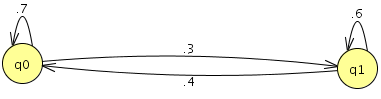
\includegraphics[height=40mm]{5_6.png}
    \begin{eqnarray*}
      P & = & \left[\begin{array}{c c}
        .7 & .3\\
        .4 & .6
      \end{array}\right]\\
      P^4 & = & \left[\begin{array}{c c}
        .5749 & .4251\\
        .5668 & .4332
      \end{array}\right]\\
      P^8 & = & \left[\begin{array}{c c}
        .572 & .428\\
        .570 & .430
      \end{array}\right]\\
    \end{eqnarray*}
    The matrix elements appear to converge and the rows become almost 
    identical. Why?\\
    \begin{definition}
      State $i$ has \underline{period} $d$ if $P^{n}_{ii} > 0$, then $d | n$ and
      $d$ is the largest of such positive integer.
    \end{definition}
    \noindent\underline{Example}: Simple symmetrical random walk on $\mathbb{Z}$.\\
      The period of any state is 2 because you can return to original position 
      if you can walk forth $k$ steps and walk back $k$ steps where $k \ge 1$.\\

    \noindent\underline{Example}: Random walk on a square. Again, $2$ because you
      can walk around the square or walk forth and back.\\

    \noindent\underline{Example}: Random walk on a triangle. 1 because you can
    return in 2 steps (walk out and back) or 3 steps (walk around the triangle).\\ 

  \noindent It can be shown that a period is the same for all states in the same
    class. If a state has period 1, it is called \underline{aperiodic}. If the chain
    is irreducible, we call it aperiodic if all state have period 1.


\section*{5/8}
  \subsection*{Periods}
    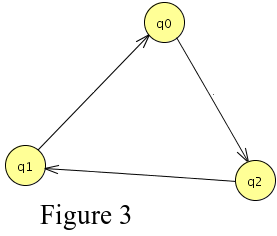
\includegraphics[width=50mm]{5_8_f3.png}
    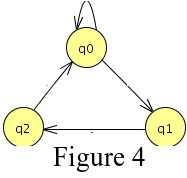
\includegraphics[width=50mm]{5_8_f4.png}\\
    \underline{Example}: Random walk on a undirected square. You have a period of 2.\\
    \underline{Example}: Random walk on a deterministic Chain (figure 3)
      You have a period of 3.\\
    \underline{Example}: Random walk on a undirected triangle. You have a period of 1.\\
    \underline{Example}: Random walk on a deterministic Chain with a chain(figure 4).
      Period is 1.\\
   
   \noindent Let $R_i = \min\{n \ge 1 | X_n = i\}$ or the first time after time 0, that
     the chain is in $i$.\\
     Also, let $f_i^n = P(R_i = n | X_0 = i)$ or the probability that the return time
     to $i$ equals $n$.\\
     Let $f_i = \sum_{n = 1}^{\infty} f_i^n$, which is the $P(\text{ever reenter $i$} |
     X_0 = i)$, so if the chain is recurrent, $\sum_{n = 1}^{\infty}f_i^n = 1$.\\
     \begin{eqnarray*}
      m_i & = & E[R_i | X_0 = i]\\
        & = & \sum_{n = 1}^{\infty} nf_i^n\\
     \end{eqnarray*}
     If $m_i < \infty$, then the series above converges and $i$ is 
     \underline{positive recurrent}.\\
     In this case, the chain is at $i$ every $m_i$ times on average.\\
    \begin{theorem}
      Assume that the chain is irreducible and positive recurrent. Let
      $N_n(i)$ be the number of visits to $i$ in the time interval between
      0 and $n$. Then,
      $$
        \lim_{n \to \infty} \frac{N_n(i)}{n} = \frac{1}{m_i}
      $$
      the former expression is the proportion of time spent at $i$.\\
    \end{theorem}
    \underline{Note}: Very trivial theorem because you need $N_n(i)$ to get
    $m_i$.\\
    \underline{Fact}: Positive recurrent in class property. An irreducible
    chain is positive recurrent if each of its states is. A finite reducible
    chain is always positive recurrent\\
    \begin{theorem}
      An irreducible positive recurrent Markov Chain has a unique 
       \underline{invariant} (aka Stationary distribution. This is a vector
       of possibilities, $\pi_i$ where $i = \{0, 1, 2, \ldots\}$.\\
       $\sum \pi_i = 1$ so that
       $$
        \sum_{\pi_i}P_{ij} = \pi_j \Leftrightarrow [\pi_0, \pi_1, \ldots]
        \cdot = [\pi_0, \pi_1, \ldots]
       $$
       So, $[\pi_0, \pi_1, \ldots]$ is the \underline{left eigenvector} of
       $P$ (for eigenvalue 1). This means that $P(X_0 = i) = \pi_i$ implies
       $P(X_n = i) = \pi_i$. Moreover,
       $$
        \pi_i = \frac{1}{m_i}
       $$
       In fact, an irreducible chain is positive recurrent $\Leftrightarrow$
       a stationary distribution exists.
    \end{theorem}
    \begin{theorem}
      If a Markov Chain is irreducible/aperiodic and positive recurrent, then
      \begin{eqnarray*}
        \lim_{n \to \infty} P_{ij}^n & = & \lim_{n \to \infty} 
          P(X_n = j | X_0 = i)\\
         & = & \pi_j \text{ (no matter what $i$ is)}
      \end{eqnarray*}
    \end{theorem}
    In summary, for finite chains,
    \begin{enumerate}
      \item $\frac{1}{n}N_n(i) \to \pi_i$ $\forall i$
      \item If the chain is aperiodic, 
        $$
          P_{ij}^n \to \pi_j
        $$
        In other words, the matrix $P^n$ eventually looks like
        $$
          \left[
          \begin{array}{c c c c}
            \pi_0 & \pi_1 & \pi_2 & \ldots\\
            \pi_0 & \pi_1 & \pi_2 & \ldots\\
            \vdots & & & \\
          \end{array}
          \right]
        $$
      \item If the chain is aperiodic with period $d$, then
        $\forall i,j$ $\exists r$
        $$
          \lim_{m \to \infty} P_{ij}^{md + r} = d\pi_j
        $$
        For all $n$ such that $n \not= r (\mod d)$,
        $P_{ij}^n = 0$
    \end{enumerate}
  \underline{Example}:
  $$
    P = \left[
    \begin{array}{c c}
      \alpha & 1 - \alpha \\
      \beta & 1 - \beta
    \end{array}
    \right]
  $$
  where $ 0 < \alpha, \beta < 1$
  \begin{enumerate}
    \item 
    $$
      \lim_{n \to \infty} P_{01}^n = \lim_{n \to \infty} 
      P(X_n = 1 | X_0 = 0) = \pi_1
    $$
    \item 
    \begin{eqnarray*}
      \pi_0\alpha + \pi_1 \beta & = & \pi_0\\
      \pi_0(1 - \alpha) + \pi_1(1 - \beta) & = & \pi_1\\
      \pi_0 + \pi_1 & = & 1\\
      &\text{ with a little algebra}&\\
      \pi_0 & = & \frac{\beta}{1 + \beta - \alpha} \\
      \pi_1 & = & \frac{1 - \alpha}{1 - \beta + \alpha}
    \end{eqnarray*}
    \item What is the time spent at 1 if $X_0 = 1$? $\pi_1$
    \item Given $X_0 = 1$, what is the expected return time to 1?
      $\frac{1}{\pi_1}$
    \item Proportion of time the chain is at 1, while the previous 
      time it was at 0? $\pi_0P_{01}$. Look at transitions.
  \end{enumerate}

\section*{5/11}
  For irreducible, finite state Markov Chains
  \begin{itemize}
    \item $\frac{N_n(i)}{n} \to \pi_i$ (irreducible)
    \item $P_{ij}^n \to \pi_j$ (irreducible, aperiodic)
  \end{itemize}
  where $[\pi_1 \ldots \pi_n]P = [\pi_1 \ldots \pi_n]$.\\

  \noindent\underline{Example}: The state of Gary\\
  (figure 5)\\
  Let Cheerful be state 0, so-so be state 1, and glum be state 2.
  Then, his transition matrix is
  $$
    P = \left(
      \begin{array}{c c c}
        .5 & .4 & .1\\
        .3 & .4 & .3\\
        .2 & .3 & .5\\
      \end{array}
    \right)
  $$
  From an initial observation, we can see it's irreducible and aperiodic.\\
  In the long run, what proportion of time is Gary in each state?
  \begin{eqnarray*}
    \pi_c + \pi_s + \pi_g & = & 1\\
    (\pi_c, \pi_s, \pi_g)P & = & (\pi_c, \pi_s, \pi_g)\\
  \end{eqnarray*}
  Solve for $Kern(P - I)^T$. This implies that $\pi_c = \frac{21}{62}$,
  $\pi_s = \frac{23}{62}$, $\pi_g = \frac{18}{62}$.\\

  \noindent\underline{Example}: The Hardy Weinberg Principle in Genetics.\\
  (Figure 6)\\
  Assume that the population has proportion, $p$ of being AA, $q$ of being
  aa, and $r$ of being Aa.\\
  Assume mating proceeds by choosing a random individual from population,
  producing 1 offspring.\\
  Let $X_n$ be genetic state of the $n^{\text{th}}$ generation.\\
  Write down $P$ and determine limiting probabilities.\\
  Let AA be state 0, aa be state 1, and Aa be state 2. Then,
  $$
    P =\left(\begin{array}{c c c}
      p + \frac{r}{2} & 0 & q + \frac{r}{2}\\
      0 & q + \frac{r}{2} & p + \frac{r}{2}\\
      \frac{p}{2} + \frac{r}{4} & \frac{q}{2} + \frac{r}{2} & 
      \frac{p}{2} + \frac{q}{2} + \frac{r}{2}\\
    \end{array}\right)
  $$
  Let $p, q, r = \frac{1}{3}$. Then,
  $$
    P =\left(\begin{array}{c c c}
    \frac{1}{2} & 0 & \frac{1}{2}\\
    0 & \frac{1}{2} & \frac{1}{2} \\
    \frac{1}{4} & \frac{1}{4} & \frac{1}{2}\\
    \end{array}\right)
  $$
  Solving for $n$, $\pi_{AA} = \frac{1}{4}$, $\pi_{aa} = \frac{1}{4}$,
  $\pi_{Aa} = \frac{1}{2}$.\\

  \noindent\underline{Example}: Random walk on a cube. Let each vertex
  of the cube be a state.\\
  Calculate $\pi_1, \ldots, \pi_8$.\\
  This is irreduicble with
  \underline{Conjecture}: 
  $$
    \pi_1 = \pi_2 = \ldots = \pi_8 = \frac{1}{8}
  $$
  Our transition matrix is
  $$
    P = \left(\begin{array}{c c c c c c c c}
    0 & \frac{1}{3} & 0 & \frac{1}{3} & \frac{1}{3} & 0 & 0 & 0\\
    \frac{1}{3} & 0 & \frac{1}{3} & 0 &0 & \frac{1}{3} & 0 & 0 \\
    & \vdots & & & & & & \\
    \end{array}\right)
  $$
  The pattern... if $i$ and $j$ are connected by an edge, then $P_{ij} =
  P_{ji}$, then $P_{ij} = P_{ji} = \frac{1}{3}$. Then, it's doubly
  stochastic. not connected by an edge, $P_{ij} = P_{ji} = 0$\\
  \begin{definition}
    Let $M$ be a square matrix. It is doubly stochastic if the sum of
    the rows is 1 and the sum of the column is 1.
  \end{definition}
  \underline{Fact}: For every doubly stochastic matrix, the invariant measure
  is $\pi_1 = \ldots = \pi_8 = \frac{1}{8}$.\\
  \begin{proof}
    We have a set of DSMs = convex hull of $\{B_1, \ldots, B_{8!}\}$, the permutation
    matrix.
    Let $M = c_1B_1 + c_2B_2 + \ldots + c_{8!}B_{8!}$ where $\sum_i c_i = 1$ where 
    $c_i \ge 0$.
  \end{proof}

\section*{5/13}
  \subsection*{Markov Chain examples continued}
    \underline{Example}: A production process can be in 4 states labeled 1, 
    2, 3, 4.\\
    On 1 or 2, it's up. Otherwise, it's down.\\
    Suppose that the transition matrix is
    $$
      P = \left(
      \begin{array}{cccc}
        \frac{1}{4} & \frac{1}{4} & \frac{1}{2} & 0\\
        0 & \frac{1}{4} & \frac{1}{2} & \frac{1}{4}\\
        \frac{1}{4} & \frac{1}{4} & \frac{1}{2} & \frac{1}{4}\\
        \frac{1}{4} & \frac{1}{4} & 0 & \frac{1}{2} \\
      \end{array}      \right)
    $$
    \begin{enumerate}
      \item Compute average length of time system remains up.
      \item Compute proportion of time system up, then down the next time.
    \end{enumerate}
    \begin{enumerate}
      \item
    If you solve
    $$
      [\pi_1, \pi_2, \pi_3, \pi_4] P = [\pi_1, \pi_2, \pi_3, \pi_4]
    $$
    with $\pi_1 + \pi_2 + \pi_3 + \pi_4 = 1$, you'll
    get $\pi_1 = \frac{3}{16}$, $\pi_2 = \frac{1}{4}$, $\pi_3 = \frac{14}{48}$,
    $\pi_4 = \frac{13}{48}$.\\
    Let $\mu$ be the average stretch of time system is up and $d$ be the average
    is down.\\
    Proportion of time up = $\frac{\mu}{\mu + d} = \pi_1 + \pi_2$.
      \item $\pi_1(P_{13} + P_{14}) + \pi_2 (P_{23} + P_{24}) = \frac{9}{32}$
        is the breakdown rate. Since there is a single breakdown in stretch of
        time up then down.
      \item Now, solve for $\mu = \frac{N}{9}$ and $d = 2$.
    \end{enumerate}

  \underline{Example}: Random walk on a graph.\\
    (figure 7)\\
    $$
    P = \left(\begin{array}{cccc}
        0 & \frac{1}{2} & \frac{1}{2} & 0\\
        \frac{1}{3} & 0 & \frac{1}{3} & \frac{1}{3}\\
        \frac{1}{3} & \frac{1}{3} & 0 & \frac{1}{3}\\
        0 & \frac{1}{2} & \frac{1}{2} & 0
      \end{array}\right)
    $$
    By symmetry, we expect $\pi_1 = \pi_4$ and $\pi_2 = \pi_3$. What do we 
    mean by symmetry?
    Let 
    $$
     Q_n = \left(\begin{array}{cccc}
      0 & 0 & 0 & 1\\
      0 & 1 & 0 & 0\\
      0 & 0 & 1 & 0\\
      1 & 0 & 0 & 0\\
      \end{array}\right)
     Q_n^{-1}
    $$
    By Symmetry, we have $Q_n^{-1}PQ_n = P$.\\
    Then, $\pi P = \pi \Rightarrow \pi Q_n^{-1}PQ_n = \pi
    \Rightarrow \pi Q_n^{-1} P = \pi Q_n^{-1}$.\\
    By uniqueness of $\pi$, $\pi = \pi Q_{n}-1 = \pi Q_{n}$.
    then, $(\pi_1, \pi_2, \pi_3, \pi_4) = (\pi_4, \pi_2, \pi_3, \pi_1)$, which
    implies that $\pi_1 = \pi_4$. Likewise, for $\pi_2 = \pi_3$.\\
    \begin{eqnarray*}
      \pi_1 & = & \frac{1}{3}\pi_2 + \frac{1}{3}\pi_3\\
      \pi_2 & = & \frac{1}{2}\pi_1 + \frac{1}{3}\pi_3 + \frac{1}{2}\pi_4\\
      \pi_3 & = & \frac{1}{2}\pi_1 + \frac{1}{3}\pi_2 + \frac{1}{2}\pi_4\\
      \pi_1 & = & \frac{1}{3}\pi_2 + \frac{1}{3}\pi_3\\
      \pi_1 = \frac{2}{3}\pi_2\\
      1 & = & 2\pi_1 + 2\pi_2\\
      \pi_2 = \frac{3}{10}\\
      \pi_1 = \frac{1}{5}\\
    \end{eqnarray*}
    \underline{Question}:
    $$
      E(\text{returned to 1} | X_0 = 1) = \frac{1}{\pi_1} = 5
    $$
    \subsection*{Renewal theory}
      Suppose $f_k \ge 0$ with $k \in \{ 1, \ldots, N \}$ such that
      $\sum_{k = 1}^N f_k = 1$.\\
      Define a Markov Chain (a renewal chain)
      (Figure 8)
      \begin{eqnarray*}
        P_{0k} & = & \frac{f_k}{1 - \sum_{l = 1}^{k} f_l} \forall k > 0\\
        P_{00} & = & f_1\\
        P_{01} & = & 1 - f_1 \\
        P_{k(k+1)} & = & \frac{P_{(k-1)k} - f_{k+1}}{P_{(k-1)k}}\\
      \end{eqnarray*}
      Suppose that $f_k$ is chosen to make chain aperiodic.\\
      For aperiocity, we require that $gcd(k, f_k > 0) = 1$.\\
      Calculate if $P($ first return to 0 is from $k$) = $f_k$, then
      $m_0 = \sum_{k=1}^N kf_k = \mu$.\\
      Calculate $P_{00}^n$ return to 0 after exactly $n$ steps.\\
      We get by conditioning to 0,
      $$
        P_{00}^n = \sum_{k = 1}^n f_k P_{00}^{n-k} \text{ for } n \le N
      $$
      Otherwise,
      $$
        P_{00}^n = \sum_{k = 1}^N f_kP_{00}^{n-k}
      $$
      Chain irreducible, aperiodic implies that
      $$
        \lim_{n \to \infty} P_{00}^n = \frac{1}{m_0} = \frac{1}{\mu}
      $$


\section*{5/15}
  \begin{theorem}[Erdos, Feller, Pollard]
  Given $f_1, \ldots f_n \ge 0$ such that $\sum_{i = 1}^N f_i = 1$.\\
  Define $\mu = \sum_{i = 1}^ni f_i$
  Assuming $gcd(k | f_k > 0) = 1$, then $\lim_{n \to \infty} u_n = \frac{1}{\mu}$.\\
  \end{theorem}
  \underline{Example}: Roll a fair die forever. Let $S_m$ be sum of first $m$ rolls.\\
  Let $P_n = P(S_m \text{ even equals} n)$.\\
  Estimate $P_{10000}$.\\
  \begin{eqnarray*}
    P_n & = & 0 \\
    P_0 & = & 1 \\
    & \vdots & \\
    P_n & = & \frac{1}{6}(P_{n-1} + \ldots + P_{n-6})\\
    f_k & = & \frac{1}{6} \text{ for } k \in \{ 1, \ldots, 6\}\\
    \mu & = & \sum_{i = 1}^6 \frac{i}{6}\\
      & = & \frac{7}{2}
  \end{eqnarray*}
  Then, 
  $$
    \lim_{n \to \infty} P_n = \frac{1}{\mu} = \frac{2}{7}
  $$
  \subsection*{Parrondo's Paradox}
    Consider games, $A, B, C$ with parameters, $p, p_1, p_2, \gamma$, which
    are each probabilities themselves and $M \ge 2$.\\
    \underline{Game A}: assymetric simple random walk
    \begin{itemize}
      \item + 1 to capital with probability $p$
      \item - 1 to capital wiht probability $1 - p$
    \end{itemize}
    Losing game if $p < \frac{1}{2}$.\\
    \underline{Game B}: Winning probabilities depend on whether your capital
    is divisible by $M$.\\
    If $M | capital$, then + 1 with probability $p_1$ and - 1 with probability 
    $1 - p_1$.\\
    If $M \not| capitals$, then +1 with probability $p_2$ and -1 with probability
    $1 - p_2$.\\
    \underline{Game C}: At each step with probability $\gamma$ play game A and
    probability $ 1 - \gamma$ to play game B.\\
    \underline{Question}: If A and B are losing, can $C$ be winning? Yes!\\
    First, we analyze game B.\\\\
    \begin{center}\underline{Analysis of Game B}\end{center}
    By Gambler's ruin, $M < x < 2M$,
    $$
      P_x(\text{walk hits $2M$ before M}) = \frac{1 - \left(\frac{1 - P_2}{P_2}
      \right)^x}{1 - \left(\frac{1 - P_2}{P_2}\right)^M}
    $$
    Starting on a multiple of $M$,
    $$
      P_M = P_1 \frac{1 - \left(\frac{1 - P_2}{P_2}\right)}{1 - \left(\frac{1
      - P_2}{P_2}\right)^M}
    $$
    Call the equation above, (1).\\
    The probability that you decrease your capital by $M$ before increasing by $M$ or
    returning to initial point is 
    $$
      (1 - p_1) \frac{\left(\frac{1 - P_2}{P_2}\right)^{M-1} - 
      \left(\frac{1 - P_2}{P_2}\right)^M}{1 - \left(\frac{1 - P_2}{P_2}\right)^M}
    $$
    Call the equation above, (2).\\
    So, game B is losing if $(2) / (1) > 1$ or equivalently,
    $$
      \frac{(1 - p_1)(1 - p_2)^{M - 1}}{P_1 P_2^{M - 1}} > 1
    $$
    \begin{center}\underline{Analysis of Game C}\end{center}
    Observe that it is the same as game B with probability
    \begin{eqnarray*}
      q_1 & = & \gamma p + (1 - \gamma) p_1\\
      q_2 & = & \gamma p + (1 - \gamma) p_1\\
    \end{eqnarray*}
    So, C is winning if
    $$
      \frac{(1 - q_1)(1 - q_2)^{M - 1}}{q_1 q_1^{M -1}} < 1
    $$
    Choosing $p = \frac{5}{11}$, $p_1 = \frac{1}{11^2}$, $p_2
    = \frac{10}{11}$, $\gamma = \frac{1}{2}$, and $M = 3$ gives
    $\frac{6}{5} > 1$ for game B. Basically, you lose.\\
    For game C, $\frac{217}{300} < 1$, so win.

\section*{5/18}
  \subsection*{pattern in coin tosses}
    Coin with heads probability, $p$. Toss is repeatedly to get a sequence of
    1s and 0s. Fix a pattern, say 1011101.\\
    \underline{Waiting Game}: What is the expected number of tosses before you
    get the pattern?\\
    \underline{Horse race}: Two patterns say 1001 and 0100. What is the 
    probability that 1001 appears first?\\
    \underline{Markov Chain}: Fix an $l$. State spaces all patterns of length $l$.
    Transition rule: the Markov Chain keeps track of the last $l$ symbols in coin
    tosses.\\
    Start with some distribution of patterns of length $l$.\\
    Invariant distribution is very simple. Would be annoying to write the transition
    matrix ($2^l$ states!).\\
    Let $n \le l$, the tosses $n + 1$, $n + 2$, $\ldots$, $n + l$ are independent
    of the starting pattern.\\
    Therefore, for any pattern, $A$, of length $l$,
    $$
      \pi_A = p^k(1 - p)^{l-k}
    $$
    where $k$ is the number of 1s in $A$.\\
    Assume that $B$ and $A$ are arbitrary patterns. Let $N_{B \to A}$ be the
    number of times that the coin needs to be tossed from $B$ to get $A$. You
    have to toss at least once.\\

    \noindent \underline{Example}: Let $B = 111001$ and $A = 110$.\\
      $111001 \to 110011 \to 100110$, so $N_{B \to A} = 2$\\
      $111001 \to 110010 \to 100100 \to 001001 \to 010011 \to 100111 \to 
      001110$, so $N_{B \to A} = 6$\\
   
    \noindent \underline{Example}: We can reformulate the waiting game to
    $$E(\emptyset \to 1011101)$$
    For any pattern $A$, we know that
    $$
      E(A \to A) = \frac{1}{\pi_A}
    $$

    \noindent\underline{Example}: $E(1011101 \to 1011101) = E(101 \to 1011101) = 
    \frac{1}{\pi_{1011101}}$\\
    The 101 above that is both at the beginning and the ending is 101 is called
    an overlap.\\
    $$
      E( \emptyset \to 1011101 ) = E( \emptyset \to 101) + E(101 \to 1011101)
    $$
    \begin{eqnarray*}
      E(\emptyset \to 101) & = & E(\emptyset \to 1) + E(1 \to 101)\\
        & = & \frac{1}{p} + \frac{1}{\pi_{101}}\\
      E( \emptyset \to 1011101 )  & = & \frac{1}{\pi_1} + \frac{1}{\pi_101} + 
        \frac{1}{\pi_{1011101}}\\
      & = & \frac{1}{p} + \frac{1}{p^2(1 - p)} + \frac{1}{5}
    \end{eqnarray*}

    \noindent\underline{Horse Race}: Let $A$ and $B$ patterns.\\
    $$
      P_A = P(A\text{ win}) \text{ and } P_B = P(B \text{ wins})
    $$
    Let $N$ be the time that the first of the two patterns appears.\\

    $$
      E(\emptyset \to A) = E(N) + p_B E(N_{B \to A})
    $$
    $(N_{\emptyset \to A} = N + I\{B \text{ wins}\} N_{B \to A})$\\
    $E( \emptyset \to B) = E(N) + p_A E(A \to B)$\\
    Then, $1 = p_a + p_b$.\\
    For $p = \frac{1}{2}$ and $A = 1001$ and $B = 0100$.\\
    $$
      E(\emptyset \to A) = 16 + 2 = 18
    $$
    $$
      E(\emptyset \to B) = 16 + 2 = 18
    $$
    $$
      E(B \to A) = E(100 \to 1001) = E(\emptyset \to 1001) - 
      E(\emptyset \to 100) = 18 - 8 = 10
    $$
    $$
      E(A \to B) = 18 - 4 = 14
    $$
    Solve the system:
    $$
      p_A = \frac{5}{12}, p_B = \frac{7}{12}, E(N) = \frac{73}{6}
    $$

    \noindent\underline{Example}:
      $A = 1010$, $B = 0100$\\
      \begin{eqnarray*}
        E(\emptyset \to A) & = & 20\\
        E(\emptyset \to B) & = & 18\\
        p_A & = & \frac{9}{14}\\
      \end{eqnarray*}
      A wins at the horse race, but loses at the waiting game. Why?
      A probably wins more, but when loses, loses badly.\\

    \noindent\underline{Example}:
      $A = 011$, $B = 100$, $C = 001$\\
      \begin{eqnarray*}
        P(A \text{ beats} B) = \frac{1}{2}
        P(B \text{ beats} C) = \frac{3}{4}
        P(C \text{ beats} A) = \frac{2}{3}
      \end{eqnarray*}

\section*{5/22}
  \underline{Example}: Random walk on the graph: The walker chooses a neighbor at 
    random, then moves there. What is the proportion of time spent at 0.

  \subsection*{Reversible Markov Chain}
    Assume that a chain starts in the invariant distribution, $X_0, X_1, \ldots,
    X_n$ has the same statistics on the time-reversal as $X_n, X_{n-1}, \ldots,
    X_0$, then we call the chain \underline{reversible}.
    Formally, we can define such chains as follows:
    $$
      P(X_{m} = j | X_{m-1} = i) = P(X_{m-1} = j | X_m = i)
    $$
    Moving forwards = Moving backwards.\\

    Let $\pi_i$ be the invariant distribution and let $\pi_i$ be the initial
    distribution, then equation says that $P_{ij} = \frac{P(X_{m-1}) = j, 
    X_m = i}{P(X_m = i)} = P(X_{m-1} = j) P(X_{m} = i | X_{m - 1} = j) = 
    \frac{\pi_jP_{ji}}{\pi_i}$.\\

    A Markov Chain is reversible with respect to invariant distribution $\pi_i$
    when $\pi_i P_{ij} = \pi_j P_{ji}$.\\

    \begin{proposition}
    If a probability mass function, $\pi_i$ satisfies
    $\pi_iP_{ij} = \pi_jP_{ji}$, then it is automatically invariant.
    \end{proposition}
    \begin{proof}
      Need to check $\pi_j = \sum_i \pi_i P_{ij}$.\\
      We know that $\sum_i \pi_i P_{ij} = \sum_i \pi_j P{ji}
      = \pi_j \sum_{i}^n P_{ji} = \pi_j D$\\
      More general problem: Assign nonnegative weights to any edge in
      a complete graph, $w_{ij} = w_{ji}$ is the weight of the edge
      between $i$ and $j$.\\
      When in $i$, the walker goes to $j$ with probability 
      proportional to $w_{ij}$, so $P_{ij} = \frac{w_{ij}}{\sum_j
      w_{ij}}$.\\
      $$
        \pi_i = \frac{\sum_j w_{ij}}{\sum_{i,j} w_{ij}}
      $$
      is a reversible measure. why? $\pi_i P_{ij} = \pi_j P_{ji}$.
      This is equivalent to $\sum_j w_{ij} \frac{w_{ij}}{\sum_j 
      w_{ij}} = \sum_i w_{ij} \frac{w_{ij}}{\sum_i w_{ij}}$.\\
    \end{proof}
    \underline{Remark}: This chain is irreducible exactly when the
      graph with edge\{$i$, $j$\} whenever $w_{ij} > 0$ is connected.
      Aperiodic $\Leftrightarrow$ not bipartite.\\

    \noindent \underline{Example}: Back to the walker problem.\\
      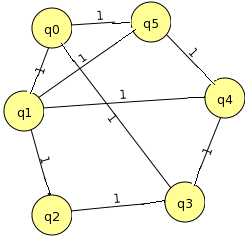
\includegraphics[height=50mm]{figure_9.png}\\
      \begin{eqnarray*}
        \pi_0 & = & \frac{3}{18}\\
        \pi_1 & = & \frac{3}{18}\\
        \pi_2 & = & \frac{3}{18}\\
        \pi_3 & = & \frac{3}{18}\\
        \pi_4 & = & \frac{3}{18}\\
        \pi_5 & = & \frac{3}{18}\\
      \end{eqnarray*}
      Therefore, proportion of time spent at 0 is $\frac{1}{6}$.\\
      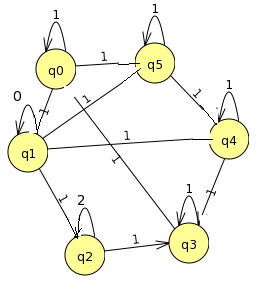
\includegraphics[height=60mm]{figure_10.png}\\

    \noindent \underline{Example}: Ehrenfest chain\\
      $M$ balls, two urns. Each time, pick a ball at random, move it from one urn to
      another.\\
      Let $X_n$ be the number of balls in urn 1.\\
      \begin{eqnarray*}
        P_{0, 1} & = & 1\\
        P_{M, M - 1} & = & 1\\
        P_{i, i - 1} & = & \frac{i}{M}\\
        P_{i, i + 1} & = & \frac{M - i}{M}\\
      \end{eqnarray*}
      With some intuitive guessing, you can see $\pi_i = \binom{M}{i}\frac{1}{2^M}$.\\
      Let's prove this. First, check for reversibility. Are the following true?
      \begin{eqnarray*}
        \pi_0 P_{01} & = & \pi_1 P_{10}\\
        \pi_i P_{i, i+1} & = & \pi_{i + 1} P_{i + 1, i}\\
        \pi_i P_{i, i-1} & = & \pi_{i - 1} P_{i - 1, i}\\
        \pi_M P_{M, M-1} & = & \pi_{M - 1} P_{M - 1, i}\\
      \end{eqnarray*}
      For the first equation
      \begin{eqnarray*}
        \pi_0 P_{01} & = & \pi_1 P_{10}\\
        \frac{1}{2^M} \cdot 1 & = & M \frac{1}{2^M} \cdot \frac{1}{M}\\
        1 & = & 1
      \end{eqnarray*}
      You can check the other equations, it matches.\\
      Also, note that this chain is irreducible, but not aperiodic. It has period 2.

\section*{5/27}
  \subsection*{Poisson Process}
    A \underline{counting process}, $N(t) \ge 0$ is a random process with
    \begin{enumerate}
      \item $N(t)$ is nonnegative integer values
      \item $N(t)$ increases in $t$
    \end{enumerate}
    $N(t) - N(s) = $ Number of events in $[s, t]$.\\
    $N(t)$ is right-continuous?)\\
    \begin{definition}
      A \underline{Poisson process} with \underline{rate} (aka 
      \underline{intensity}) $\lambda > 0$ is a counting process $N(t)$ such
      that
      \begin{enumerate}
        \item $N(0) = 0$
        \item It has independent increments: if $(s_1, t_1] \bigcap (s_2, t_2]
          = \emptyset$, then $N(t_1) - N(s_1)$ and $N(t_2) - N(s_2)$ are 
          independent
        \item Number of events in any interval of length, $t$, is 
          $Poisson(\lambda t)$, i.e. $P(N(t+s) - N(s) = k) = e^{-\lambda t}
          \frac{(\lambda t)^k}{k!}$, $i = 0, 1, 2, \ldots$. $E(N(t + s) - N(s))
          = \lambda t$
      \end{enumerate}
    \end{definition}
    
  \subsection*{Review of Exponential random variables}
    $X$ is $exp(\lambda)$ means that
    \begin{eqnarray*}
      f_X(x) & = & \begin{cases} \lambda e^{-\lambda x} & x \ge 0\\ 0 & x < 0 \end{cases}\\
      P(X \ge x) & = & e^{-\lambda x}, x > 0\\
      E(X) & = & \frac{1}{\lambda}\\
      Var(X) & = & \frac{1}{\lambda^2}\\
      P(X > s + t | X > t) & = & P(X > s)
    \end{eqnarray*}
    The last equation is known as the "memoryless" property.

  \subsection*{Review of Poisson random variables}
    $X$ is $Poisson(\lambda)$ means that 
    \begin{eqnarray*}
      P(X = k) & = & e^{-\lambda}\frac{\lambda^k}{k!}, k = 0, 1, \ldots\\
      EX & = & \lambda\\
      Var(X) & = & \lambda\\
    \end{eqnarray*}
    If $X_i$ is $Poisson(\lambda_i)$ and indpendent, then $X_1 + \ldots + X_n$ is
      $Poisson(\lambda_1 + \ldots + \lambda_n)$. (Superposition property)\\
    If $X$ is $Poisson(\lambda)$ and $I_i$ are independent indicators with $P(I_i
      = 1) = p$, then $\sum_{i = 1}^x I_i$ is $Poisson(\lambda p)$. (thinning 
      property)\\
    Figure 12\\
    $P(N(h) = 1) = e^{-\lambda h} \lambda h \approx \lambda h$ as $h \to 0$.\\
    $P(N(h) \ge 2) = O(h^2) < \lambda h$\\
    This is why $\lambda$ is called rate.\\\\
    In fact, we could construct a Poisson process in the following way: Any integer
    multiple of $\frac{1}{n}$.\\
    Toss a coins with heads probability $\frac{\lambda}{n}$. Mark the location of heads.\\
    Let $N_n(t)$ be the number of heads on $[0, t]$.\\
    When $n \to \infty$, $N_n(t)$ converges to a Poisson process with rate $\lambda$.\\
    Number of heads is $Binomial(nt \pm 1, \frac{\lambda}{n}) \approx Poisson(\lambda t)$.\\\\
    
    \noindent Let $T_1, T_2, \ldots$ be the \underline{interarrival times} where $T_n$ be the
    time elapses between $(n-1)'s$ and $n'th$ event. (like buses coming).\\
    \begin{proposition}
      $T_1, T_2, \ldots$ are independent and distributed $exp(\lambda)$.
    \end{proposition}
    \begin{proof}
      $P(T_1 > t) = P(N(t) = 0) e^{-\lambda t}$\\
      $P(T_2 > t | T_1 = s) = P(\text{no events in }(s, s + t] | T_1 = s) = 
      P(N(t) = 0) = e^{-\lambda t}$. It does not matter what happen between 
      0 and $s$.\\
    \end{proof}

\section*{5/29}
  \subsection*{Poisson process}
    "Tossing low probability coins very fast."\\
    Mark an $x$ at each multiple of $\frac{1}{n}$ with probability 
    $\frac{\lambda}{n}$ as $n \to \infty$
    $P(\text{number of events in interval of length $k$} \ldots$
    $T_n$ are independently and identically distributed $exp(\lambda)$ and
    $ET_n = \frac{1}{x}$.\\
    Let $S_n = T_1 + \ldots + T_n$ be the waiting time for $n^{\text{th}}$ 
    event.\\
    Compute the density of $S_n$.\\
    (We know that $ES_n = \frac{n}{\lambda}$)\\
    \begin{eqnarray*}
      P(S_n > t) & = & P(N(t) < n) = \sum_{j = 0}^{n-1} e^{-\lambda t} \frac{
      (\lambda t)^j}{j!}\\
     -f_{S_n}(t) & = & \sum_{j = 0}^{n - 1} \frac{1}{j} (-\lambda e^{-\lambda t}
     (\lambda t)^j + e^{-\lambda t} j (\lambda t)^{j - 1} \lambda)\\
     & = & \lambda e^{-\lambda t} \sum_{j = 0}^{k - 1} (-\frac{(\lambda t)^j}
     {j!} + \frac{(\lambda t)^{j - 1}}{(j-1)!}\\
     & = & - \lambda e^{-\lambda t} \frac{(\lambda t)^{n-1}}{(n-1)!}
     f_{S_n}(t) = \lambda e^{-\lambda t}\frac{(\lambda t)^{n-1}}{(n -1)!}
   \end{eqnarray*}
   Above result is called Gamma distrubtion.\\\\
   \underline{example}: Poisson process with rate $\lambda$.\\
   \begin{eqnarray*}
    E(\text{time of 10th event}) & = & \frac{10}{\lambda}\\
    P(\text{10th event occurs 2 or more time units after 9th event}) & = & e^{-2\lambda}\\
    P(\text{10th event occurs later than time 20}) & = & \int_{20}^{\infty} 
    \lambda e^{-\lambda t} \frac{(\lambda t)^9}{9!}\,dt\\
    & = & P(S_{10} > 20)\\
    & = & P(N(20) < 10)\\
    & = & \sum_{j = 0}^9 e^{-20\lambda} \frac{(20\lambda)^j}{9!}\\
   \end{eqnarray*}
   \begin{eqnarray*}
    P(\text{2 events in $[1, 4)$ and 3 events in $[3,5]$})
      & = & \sum_{k = 0}^2 P( \ldots | \text{$k$ events in $[3, 4]$}) 
        P(\text{$k$ events in $[3, 4]$})\\
      & = & \sum_{k = 0}^{2} P(\text{$2 - k$ events in $(1, 3]$ and $3 - k$
      events in $[4, 5]$)} \\
      & & P(\text{$k$ events in $[3,4]$})\\
      & = & \sum_{k = 0}^2 e^{-2\lambda} \frac{(2\lambda)^{2 - k}}{(2 - k)!}
        e^{-\lambda}\frac{\lambda^{3 - k}}{(3 - k)!} e^{-\lambda}
        \frac{\lambda^k}{k!}\\
      & = & e^{-4\lambda}(\frac{1}{3} \lambda^5 + \lambda^4 + \lambda^3)\\
   \end{eqnarray*}
   \subsection{Superposition}
    Two \underline{independent} Poisson processes with $\lambda_1$ and 
    $\lambda_2$ can be combined into a single Poisson process with rate 
    $\lambda_1 + \lambda_2$.\\
    $N_1(t) + N_2(t) = N(t)$.\\
   \subsection*{Thinning}
    Flip a coin with probability $p$ for heads for every event in a Poisson 
    process. Call Type I events for those with heads and Type II events for 
    those with tails. \\
    Let $N_1(t)$ be the number of Type I events in $[0, t]$.\\
    Let $N_2(t)$ be the number of Type II events in $[0, t]$.\\
    These are both Poisson processes with parameter $\lambda p$ and 
    $\lambda(1-p)$, respectively.\\
    Further, these two processes are independent.\\
    \underline{Idea}: Discretize.\\
      construct Type I process by flipping $\frac{p\lambda}{n}$, coins at 
      multiples of $\frac{1}{n}$. Then, construct type II process by flipping
      $\frac{\lambda(1 - p)}{n}$ coins on the remaining points. Send $n \to
      \infty$.\\

    \noindent\underline{Example}: Customer arrive at a store at rate 10/hr.
      Each are either male or female with probability $\frac{1}{2}$. Assume that
      you know that exactly 10 women entered within some hour (say 10 - 11am).
      (a) Compute the probability that exactly 10 men also entered.\\

    \noindent They're completely independent Poisson process. Parameter is
      $\frac{1}{2} \cdot  10 = 5$, so our answer is
      $$
        e^{-5} \frac{5^{10}}{10!}
      $$

    \noindent Compute the probability that at least 20 customers have entered.\\

    $$
      = \sum_{k = 10}^{\infty} P(\text{$k$ men entered}) = \sum_{10}^{\infty}
        e^{-5} \frac{5^k}{k!}
    $$

    \noindent \underline{Example}: Assume that cars arrive at rate, 10 / hr. 
      Assume each car will pick up a hitchhiker with probability $\frac{1}{10}$.
      You are 2nd in line. What is the probability tht you'll have to wait for 
      more than 2 hours?\\

    \noindent Cars that pick up are a Poisson process with rate $10 \cdot 
      \frac{1}{10} = 1$.\\
      $\lambda = 2$ because average is 1 and time is 2.
      $$
        P(T_1 + T_2 > 2) = P(N(2) \le 1) = e^{-\lambda t} (1 + \lambda t) = e^{-2}(1 + 2) = 3e^{-2}
      $$

\section*{6/1}
  Assume that you have two independent Poisson process $N_1(t)$ with rate
  $\lambda_1$ and $N_2(t)$ with rate $\lambda_2$. What is the probability that
  $n$ events occur in the first process before $m$ events occur in the 2nd
  process.\\

  \noindent \underline{Example}: $\lambda_1 = 5$, $\lambda_2 = 1$, $n = 5$,
  $m = 2$.\\
  Let $T_i^1$ be the interarrival times for the 1st process.\\
  Let $T_i^2$ be the interarrival times for the 2nd process.\\
  Let $S_n^1 = T_1^1 + \ldots T_n^1$\\
  Let $S_m^2 = T_1^2 + \ldots T_m^2$\\
  Start with a continued Poisson process with $\lambda_1 + \lambda_2$, then
  independently decide for each event whether it belongs to the 1st process
  with probability $\frac{\lambda_1}{\lambda_1 + \lambda_2}$ or the 2nd process
  with probability $\frac{\lambda_2}{\lambda_1 + \lambda_2}$. The obtained 
  processes are independent and have the correct rates.\\

  \begin{eqnarray*}
    P(S_n^1 < S_m^1) & = & P(\text{among first $m + n -1$ events (in the 
      combined process), $n$ or more events belong to the 1st process})\\
      & = & \sum_{k = n}^{n + m -1} \binom{n + m -1}{k} \left(\frac{\lambda_1}
      {\lambda_1 + \lambda_2}\right)^k 
      \left(\frac{\lambda_2}{\lambda_1 + \lambda_2}\right)^{n + m - 1 - k}\\
      & = & \sum_{k = 5}^6 \binom{6}{k} \left(\frac{5}{6}\right)^k\left(\frac
        {1}{6}\right)^{6 - k}\\
      & = & \frac{11 \cdot 5^5}{6^6}
  \end{eqnarray*}
  If you change $m = 1$, then our answer is $\left(\frac{5}{6}\right)^5$\\

  \noindent \underline{Example}: You have 3 friends, $A, B, C$. Each will call
    you on exponential amount of time with $exp(30min), exp(1hr), exp(2.5hr)$
    respectively. You will go out with the first one that calls. What is
    the probability that you go out with $A$?\\

  \noindent Intepret each call as the first event in a Poisson process (rates
    $2, 1, \frac{5}{2}$ (the units are an hour)). Note that rates are inverses
    of your mean.\\

  \noindent Let the rates be $\lambda_1, \lambda_2, \lambda_3$ respectively.\\
    Start with ($\lambda_1 + \lambda_2 + \lambda_3$) Poisson process, distribute
    the events with probability $\frac{\lambda_1}{\lambda_1 + \lambda_2 + 
    \lambda_3}$, $\frac{\lambda_2}{\lambda_1 + \lambda_2 + \lambda_3}$, and
    $\frac{\lambda_3}{\lambda_1 + \lambda_2 + \lambda_3}$ respectively.\\
    Probability of A calling first is $\frac{\lambda_1}{\lambda_1 + \lambda_2 +
    \lambda_3} = \frac{2}{2 + 1 + \frac{5}{2}}$.\\

  \begin{theorem}
    Given that $N(t) = k$, the conditional distribution of the arrival times,
    $S_1, \ldots, S_k$, is distributed as order statistics of $k$ independent
    uniform variables: the set $\{ S_1, \ldots, S_k\} = \{U_1, \ldots, U_i\}$,
    where $U_i$ are iid uniform on $[0, t)$.\\
  \end{theorem}
  \begin{theorem}
    Given that $S_k = t$, $S_1, \ldots, S_{k - 1}$ are distributed as order 
    statistics of $k - 1$ uniform $(0, t)$ random variables.\\
  \end{theorem}
  \begin{proof}
    Why? $N$ independently coins with heads probability $p$. Condition on
    $k$ heads.\\
    \begin{eqnarray*}
      P(k \text{ heads occurs on specifics subset of $k$ coins} | \text{$k$ 
      heads}) & = & \text{same for all subsets of size $k$}\\
    \end{eqnarray*}
  \end{proof}

  \noindent \underline{Example}: Assume that passangers arrive as a Poisson
  process with rate $\lambda$.
  \begin{enumerate}
    \item The only bus departs after time $T$. Compute the expected combined 
      walking time, $W$ for all passangers.\\

      \noindent If $S_1, S_2, \ldots, $ are the arrival times in $[0, 1]$, then
      the combined waiting times, $T - S_1 + T - S_3 + \ldots$\\
      Let $N(t)$ be the number of arrivales in $[0, t]$.\\
      \begin{eqnarray*}
        E(W) & = & \sum_{k = 0}^{\infty}E[W | N(T) = k] P(N(T) = k)\\
        & = & \sum_{k  = 0}^{\infty} \ldots
      \end{eqnarray*}
    \item now, two buses depart, are at $T$, one at $S < T$, $EW$
      
      \noindent $\lambda \frac{s^2}{2} + \lambda \frac{(T - S)^2}{2}$

    \item Now assume $T$(the only bus time) is $exponential(\mu)$, indpendent
    of the passengers.\\

      \noindent 
        \begin{eqnarray*}
          EW & = & E(W | T = t)E(T = t)\\
            & = & \int_0^{\infty} \lambda\frac{t^2}{2}f_T(t)dt\\
            & = & \frac{\lambda}{2} E(T^2)\\
            & = & \frac{\lambda}{2} (Var(T) + (ET)^2)\\
            & = & \frac{\lambda}{2} \frac{2}{\mu^2}\\
            & = & \frac{\lambda}{\mu^2}
        \end{eqnarray*}
    \item Two busses now arrive as first two events in a $poisson(\mu)$ process
    $EW = 2\frac{\lambda}{\mu^2}$
  \end{enumerate}

\section*{6/3}
  \underline{Exercise 7.9}
    You have two machines. $M_1$ has lifetime $exp(\lambda_1)$ and $M_2$
    has lifetime $exp(\lambda_2)$. Let their lifetimes be $T_1$ and $T_2$.\\
    Machine 1 starts at time 0 and Machine 2 starts at time $t$.
    \begin{eqnarray*}
      P(\text{Machine 1 is the 1st to fail}) 
      & = & P(T_1 < T_2 + t)\\
      & = & P(T_1 < t)  + P(T_1 \ge t, T_1 < T_2 + t)\\
      & = & P(T_1 < t) + P(T_1 < T_2 + t |] T_1 \ge t) P(T_1 \ge t)\\
      & = & 1 - e^{-\lambda_1 t} + P(T_1 - t < T_2 | T_1 \ge t) e^{-\lambda_1 t}\\
      & = & 1 - e^{-\lambda_1 t} + P(T_1 < T_2) e^{-\lambda_1 t} \text{ (Memoryless probability.)}\\
      & = & 1 - e^{-\lambda_1 t} + \frac{\lambda_1}{\lambda_1 + \lambda_2} 
        e^{-\lambda_1 t} \text{ (Poisson process)}
    \end{eqnarray*}
    What if we replace $t$ with $T$, exponential (and independent of $T_1, T_2$)
    with parameter $\mu$?\\
    \begin{eqnarray*} 
      P(T_1 < T_2 + T)
      & = & P(T_1 < T) + P(T_1 \ge T, T_1 < T_2 + T)\\
      & = & \frac{\lambda_1}{\lambda_1 + \mu} + \frac{\lambda_1}{\lambda_1 + 
        \lambda_2}\frac{\mu}{\lambda_1 + \lambda_2}\\
    \end{eqnarray*}
  \underline{Example}: Hitchhiker's problem. You have $A$ and $B$. Cars that
  would pick up a hitchhiker approximately at a Poisson process at rate 
  $\lambda_0$. $A$ is first in line.\\
  After $exp(\lambda_A)$ time, $A$ quits.\\
  After $exp(\lambda_B)$ time, $B$ quits.\\
  \begin{eqnarray*}
    P(\text{A gets picked})
    & = & \frac{\lambda_{c}}{\lambda_{A} + \lambda_{c}}\\
    P(\text{B gets picked})
    & = & P(\text{at least 2 cars arrives before B quits} \bigcup \text{A quits
    and at least one car arrives before B quits})\\
    & = & P(\text{at least 2 cars arrives before B quits}) + P(\text{A quits
    and at least one car arrives before B quits}) - P(\text{A quits and at least
    2 cars arrive before B quits})\\
    & = & \left(\frac{\lambda_c}{\lambda_B + \lambda_c}\right)^2 + \left(
      \frac{\lambda_A}{\lambda_A + \lambda_B + \lambda_c}\right) \left(
      \frac{\lambda_c}{\lambda_A + \lambda_B + \lambda_c}\right) - \left(
      \frac{\lambda_A}{\lambda_A + \lambda_B + \lambda_c}\right) \left(
      \frac{\lambda_c}{\lambda_A + \lambda_B + \lambda_c}\right)^2\\
    & = & \frac{\lambda_A + \lambda_c}{\lambda_A + \lambda_B + \lambda_C} \cdot
      \frac{\lambda_C}{\lambda_B + \lambda_C}
  \end{eqnarray*}
  Better way:
  \begin{eqnarray*}
    P(\text{B gets picked})
    & = & P(\text{first event is either $A$ or $C$ and next event among $B$ and
      $C$ only has to be C})
  \end{eqnarray*}


\end{document}
